\chapter{Additional Exercises}
The aim of this chapter is to provide more realistic problems that can be solved using \mlab. The questions are adapted from \gilatbook
\section{Basic Concepts} \label{sect:basic_concepts}
\begin{enumerate}
\item \textit{Variables}\\
An object with an initial temperature of $T_0$ that is placed at time $t=0$ inside a chamber that has a constant temperature of $T_s$, will experience a temperature change according to the equation:
\begin{equation*}
T = T_s + (T_0 - T_s)e^{-kt},
\end{equation*}
where $T$ is the temperature of the object at time $t$, and $k$ is a constant. A soda can at a temperature of 49~$^\circ$C (was left in the car) is placed inside a refrigerator where the temperature is 3~$^\circ$C. Determine, to the nearest degree, the temperature of the can after three hours. Assume $k=0.45$. First define all the variables and then calculate the temperature using one \mlab command.

\item \textit{Variables}\\
Radioactive decay is modeled with the exponential function $f(t) = f(0)e^{kt}$, where $t$ is time, $f(0)$ is the amount of material at $t=0$, $f(t)$ is the amount of material at time $t$, and $k$ is a constant. Gallium-67, which has a half-life of 3.261~days, is used for tracing cancer. If 100~mg are present at $t=0$, determine the amount that is left after 7~days. You should first determine the constant $k$ and then calculate $f(7)$. 

\item \textit{Variables}\\
The magnitude $M$ of an earthquake on the Richter scale is given by:
\begin{equation*}
M = \frac{2}{3} log_{10} \left( \frac{E}{E_0} \right),
\end{equation*}
where $E$ is the energy release by the earthquake, and $E_0 = 10^{4.4}$~J is a constant (the energy of a small reference earthquake). Determine how many more times energy is released from an earthquake that registers 7.1 on the Richter scale than an earthquake that registers 6.9.

\item \textit{Variables}\\
The temperature dependence of vapor pressure $p$ can be estimated by the Antoine equation:
\begin{equation*}
ln(p) = A - \frac{B}{C + T},
\end{equation*}
where $ln$ is the natural logarithm, $p$ is in mm Hg, $T$ is in Kelvin, and $A$, $B$, and $C$ are material constants. For toluene ($C_6H_5CH_3$) in the temperature range from 280 to 410~K the material constants are: $A = 16.0137$, $B = 3096.52$, and $C = -53.67$. Calculate the vapour pressure of toluene at 315 and 405~K.

\item \textit{Adding vectors}\\
Three forces are applied to a bracket as shown in Figure~\ref{fig:adding-forces}. Determine the total (equivalent) force applied to the bracket.
\begin{figure}[h]
	\myfloatalign
	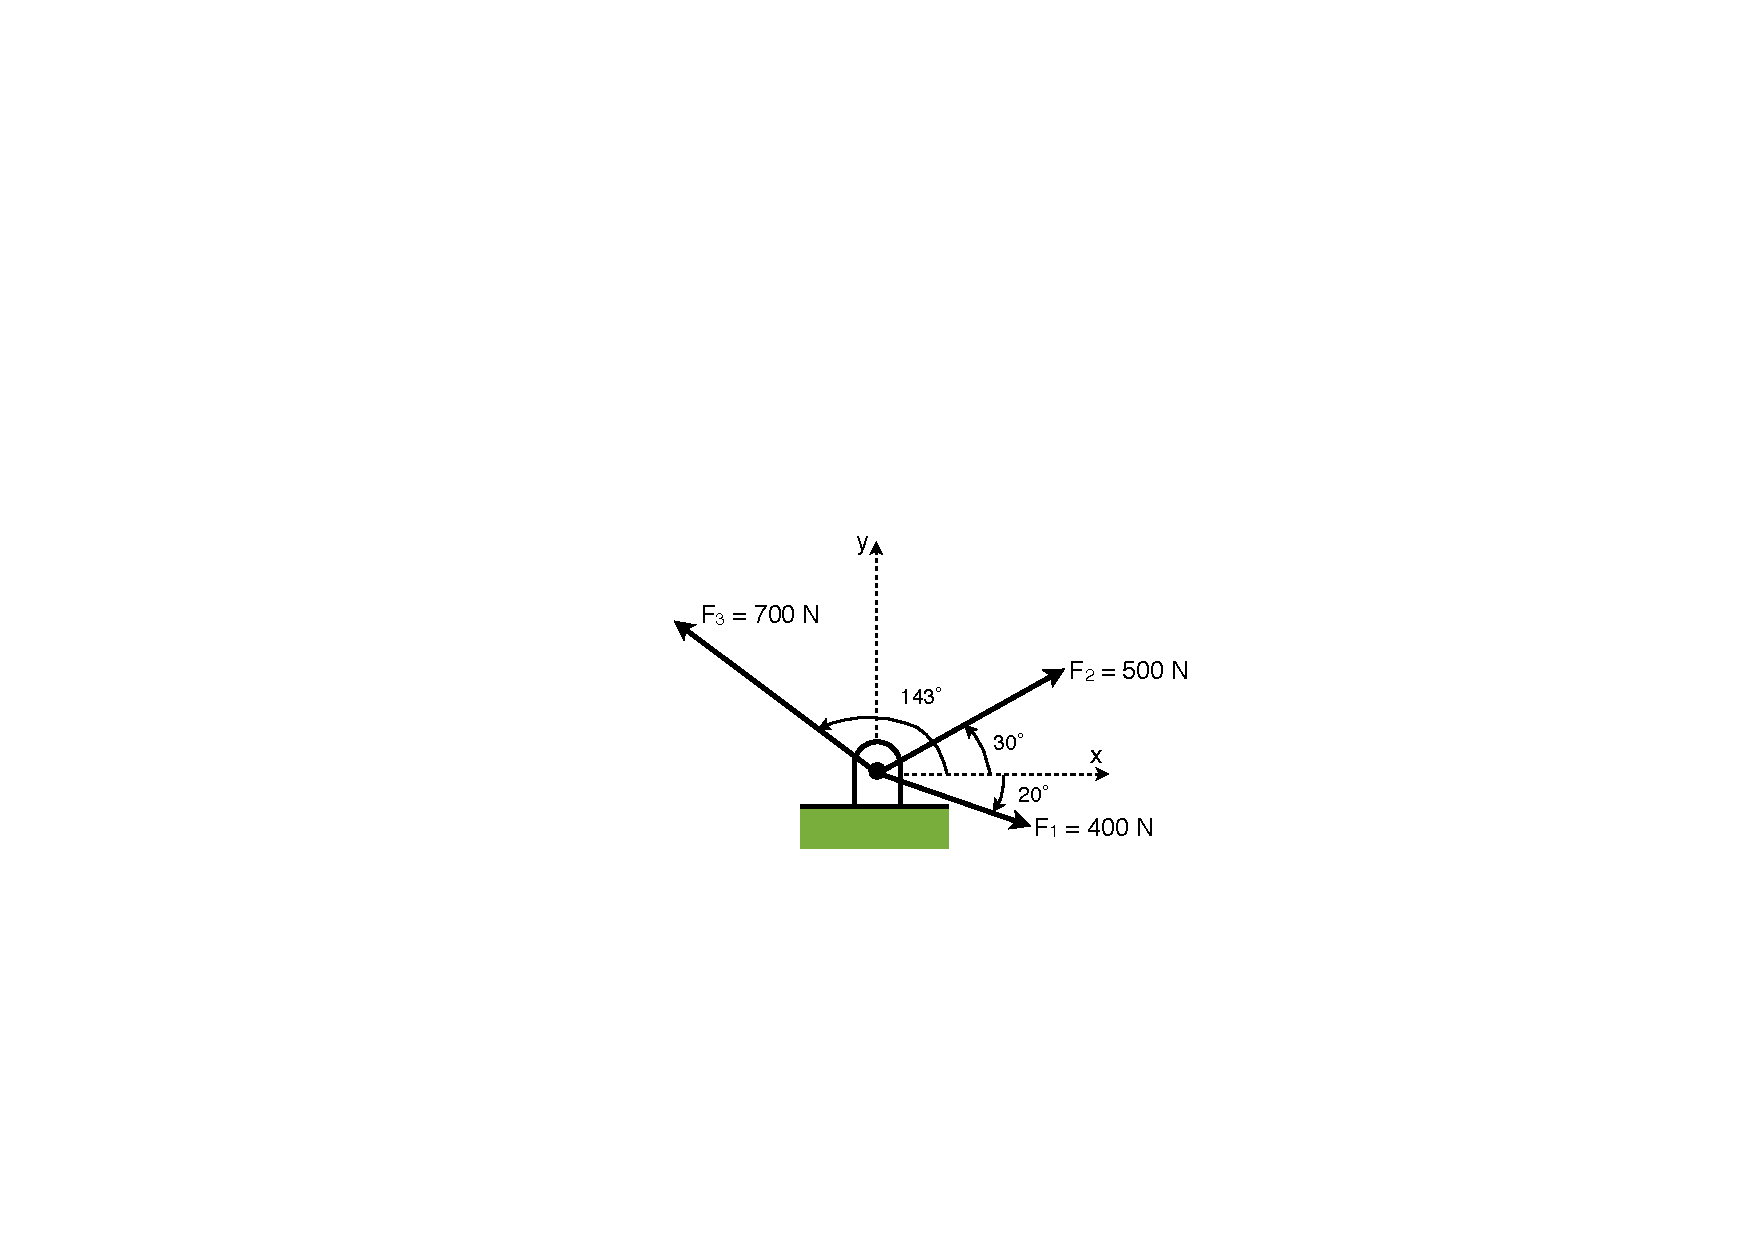
\includegraphics[width=0.65\linewidth]{Graphics/Additional-Ex/adding-forces}
	\caption{Forces on a bracket}
	\label{fig:adding-forces}
\end{figure}

\addtolength{\parindent}{-4mm}
\fcolorbox{myborderblue}{myblue}{%
\begin{minipage}{\linewidth}
\begin{minipage}{6mm}

\includegraphics[scale=0.03]{Graphics/General/help_icon}
\end{minipage}
\textit{Addition of forces in \twod space} \\
A force is a vector (physical quantity that has magnitude and direction). In a Cartesian coordinate system a \twod vector $\boldsymbol{F}$ can be written as:
\begin{equation*}
\boldsymbol{F} = F_x\boldsymbol{i} + F_y\boldsymbol{j} = Fcos(\theta)\boldsymbol{i} + Fsin(\theta)\boldsymbol{j} = F(\cos(\theta)\boldsymbol{i} + \sin(\theta)\boldsymbol{j}),
\end{equation*}
where $F$ is the magnitude of the force, and $\theta$ is its angle relative to the $x$ axis, $F_x$ and $F_y$ are the components of $\boldsymbol{F}$ in the directions of the $x$ and $y$ axis, respectively, and $\boldsymbol{i}$ and $\boldsymbol{j}$ are unit vectors in these directions. If $F_x$ and $F_y$ are known, then $F$ and $\theta$ can be determined by:
\begin{equation*}
F = \sqrt{{F_x}^2 + {F_y}^2} \quad \textrm{and} \quad \tan(\theta) = \frac{F_x}{F_y}
\end{equation*}
\end{minipage}%
}\\
\addtolength{\parindent}{4mm}

\item \textit{Element-by-element calculations}\\
The coefficient of friction $\mu$ can be determined in an experiment by measuring the force $F$ required to move a mass $m$ as shown in Figure~\ref{fig:friction}. 
\begin{figure}[h]
	\myfloatalign
	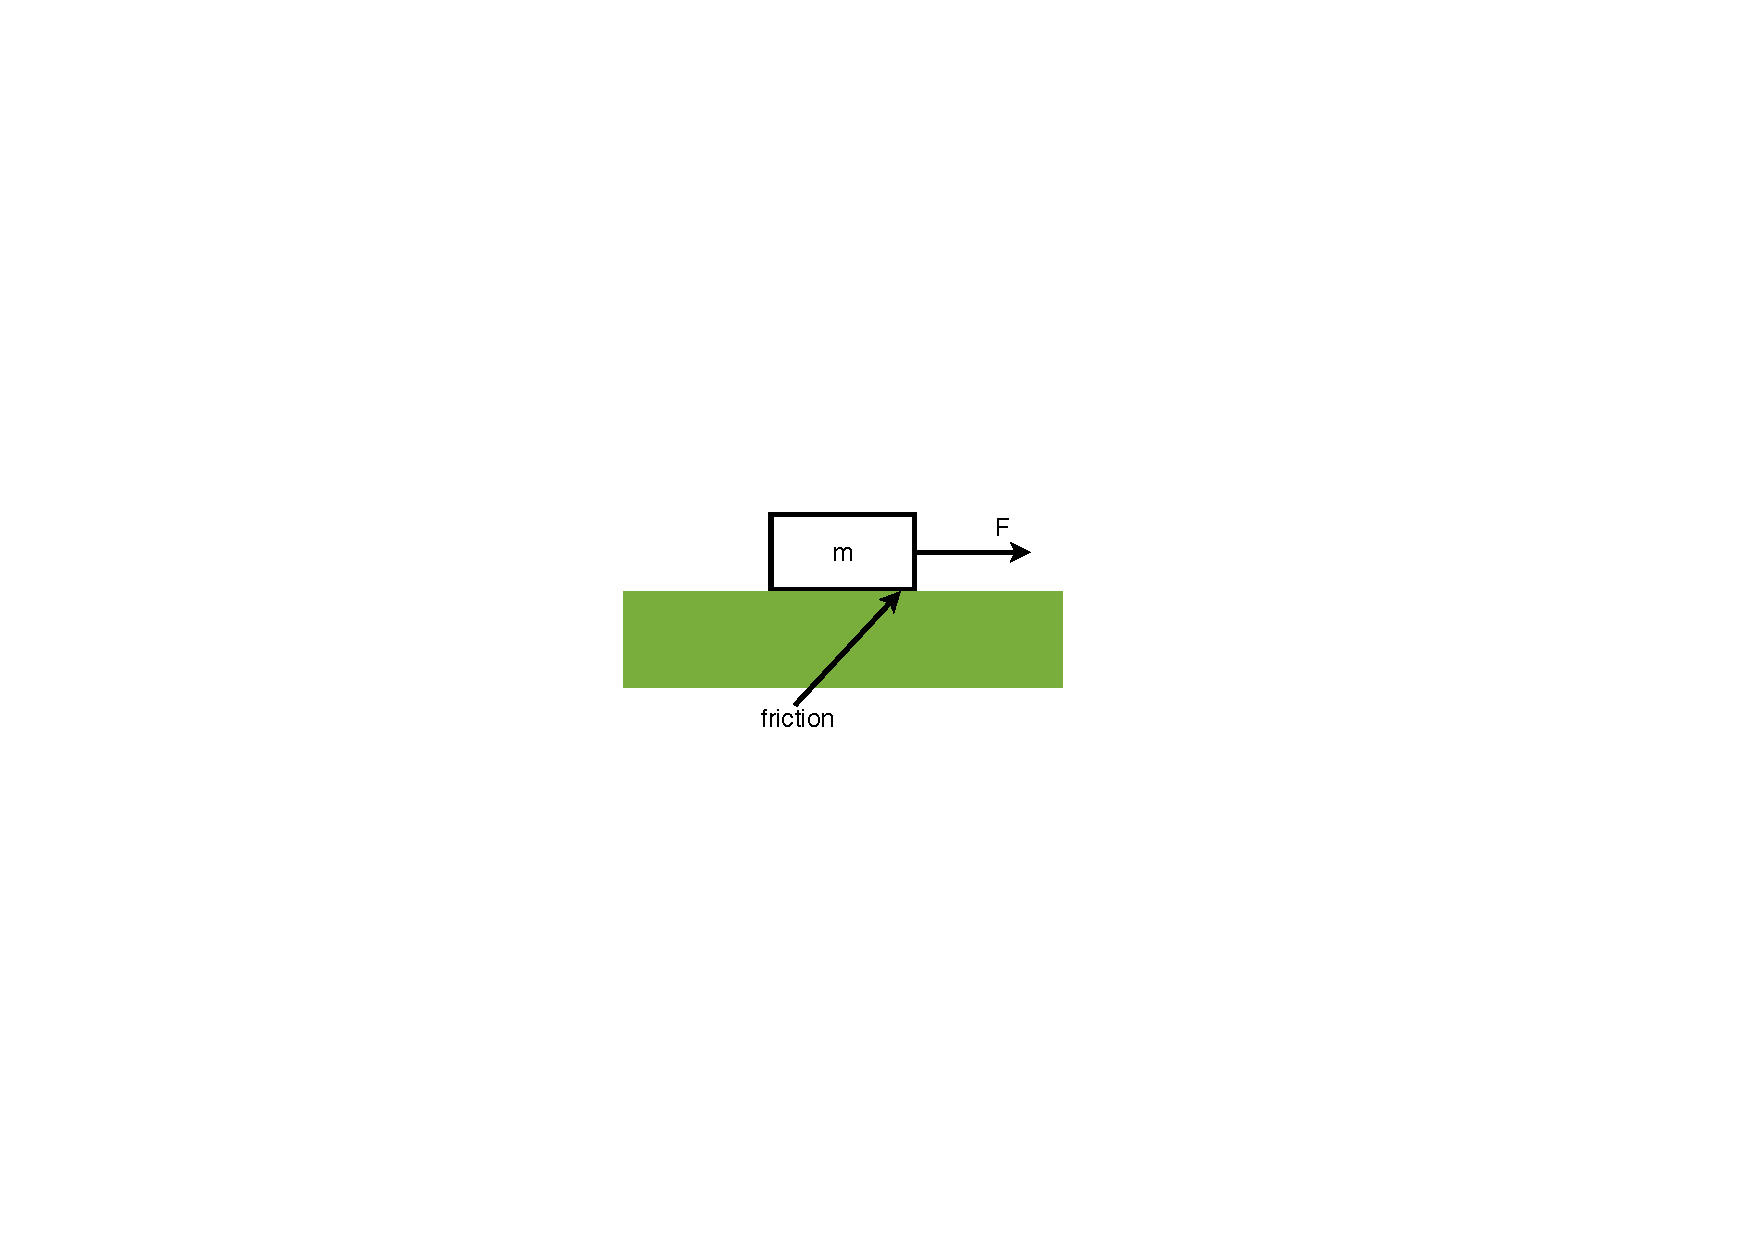
\includegraphics[width=0.55\linewidth]{Graphics/Additional-Ex/friction}
	\caption{Friction}
	\label{fig:friction}
\end{figure}
When $F$ is measured and $m$ is known, the coefficient of friction can be calculated by:
\begin{equation*}
\mu = \frac{F}{mg},
\end{equation*}
where $g = 9.81~m/s^2$. Results from measuring $F$ in six tests are given in Table~\ref{tab:friction}. Determine the coefficient of friction in each test, and the average from all tests.
\begin{table}[h]
	\caption{Friction experiment results}
	\label{tab:friction}
	\myfloatalign
	\begin{tabular}{lcccccc}\toprule
	\spacedlowsmallcaps{Test no.} & 1 & 2 & 3 & 4 & 5 & 6 \\ \midrule
	\spacedlowsmallcaps{Mass (kg)} & 2 & 4 & 5 & 10 & 20 & 50 \\
	\spacedlowsmallcaps{Force (N)} & 12.5 & 23.5 & 30 & 61 & 117 & 294 \\
	\bottomrule
	\end{tabular}
\end{table}

\item \textit{Solving linear equations}\\
The electrical circuit shown in Figure~\ref{fig:circuit} consists of resistors and voltage sources. 
\begin{figure}[h]
	\myfloatalign
	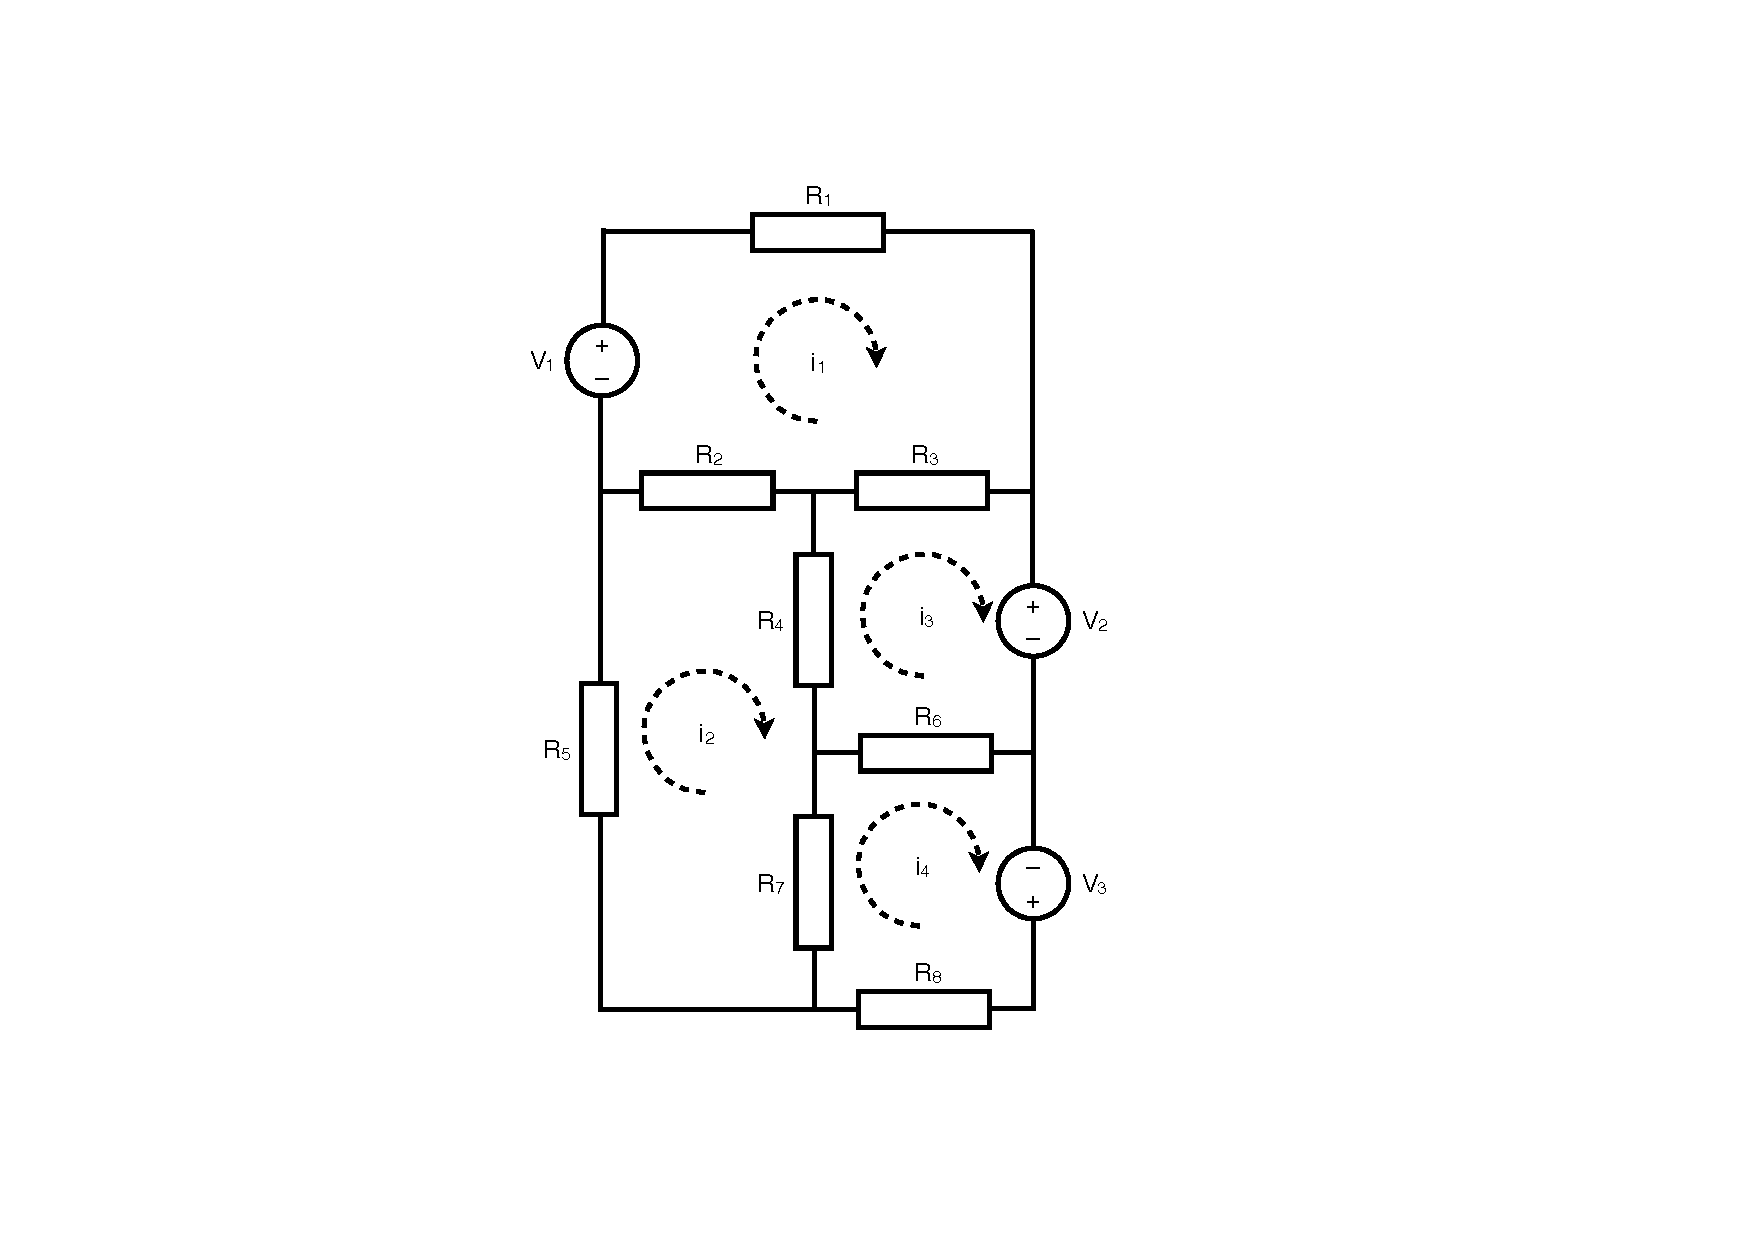
\includegraphics[width=0.65\linewidth]{Graphics/Additional-Ex/resistor-net}
	\caption{Network of voltage sources and resistors}
	\label{fig:circuit}
\end{figure}
Determine the current in each resistor using the mesh current method which is based on Kirchhoff's voltage law.
\begin{align*}
V_1 &= 20~V \quad V_2 = 12~V \quad V_3 = 40~V \\
R_1 &= 18~\Omega \quad R_2 = 10~\Omega \quad R_3 = 16~\Omega \quad R_4 = 6~\Omega \\
R_5 &= 15~\Omega \quad R_6 = 8~\Omega \quad R_7 = 12~\Omega \quad R_8 = 14~\Omega
\end{align*}
\addtolength{\parindent}{-4mm}
\fcolorbox{myborderblue}{myblue}{%
\begin{minipage}{\linewidth}
\begin{minipage}{6mm}

\includegraphics[scale=0.03]{Graphics/General/help_icon}
\end{minipage}
\textit{Kirchhoff's voltage law} \\
Kirchhoff's voltage law states that the sum of the voltage around a closed circuit is zero. In the mesh current method a current is assigned to each mesh ($i_1, i_2, i_3, i_4$). Then, Kirchhoff's voltage law is applied for each mesh, resulting in a system of linear equations for the currents (four equations in this case). The solution of the equations gives the values of the mesh currents. The current in a resistor that belongs to two meshes is the sum of the currents in the corresponding meshes. It is convenient to assume that all the currents are in the same direction (clockwise in this case). In the equation for each mesh, the voltage source is positive if the current flows to the cathode (negative electrode), and the voltage of the resistor is negative for current in the direction of the mesh current.
\end{minipage}%
}\\
\addtolength{\parindent}{4mm}

\newpage
\section{Plotting} \label{sect:plotting}
\item \textit{2D plotting}\\
In a typical tension test a dog-bone shaped specimen, as shown in Figure~\ref{fig:tension-test}, is pulled in a machine. 
\begin{figure}[h]
	\myfloatalign
	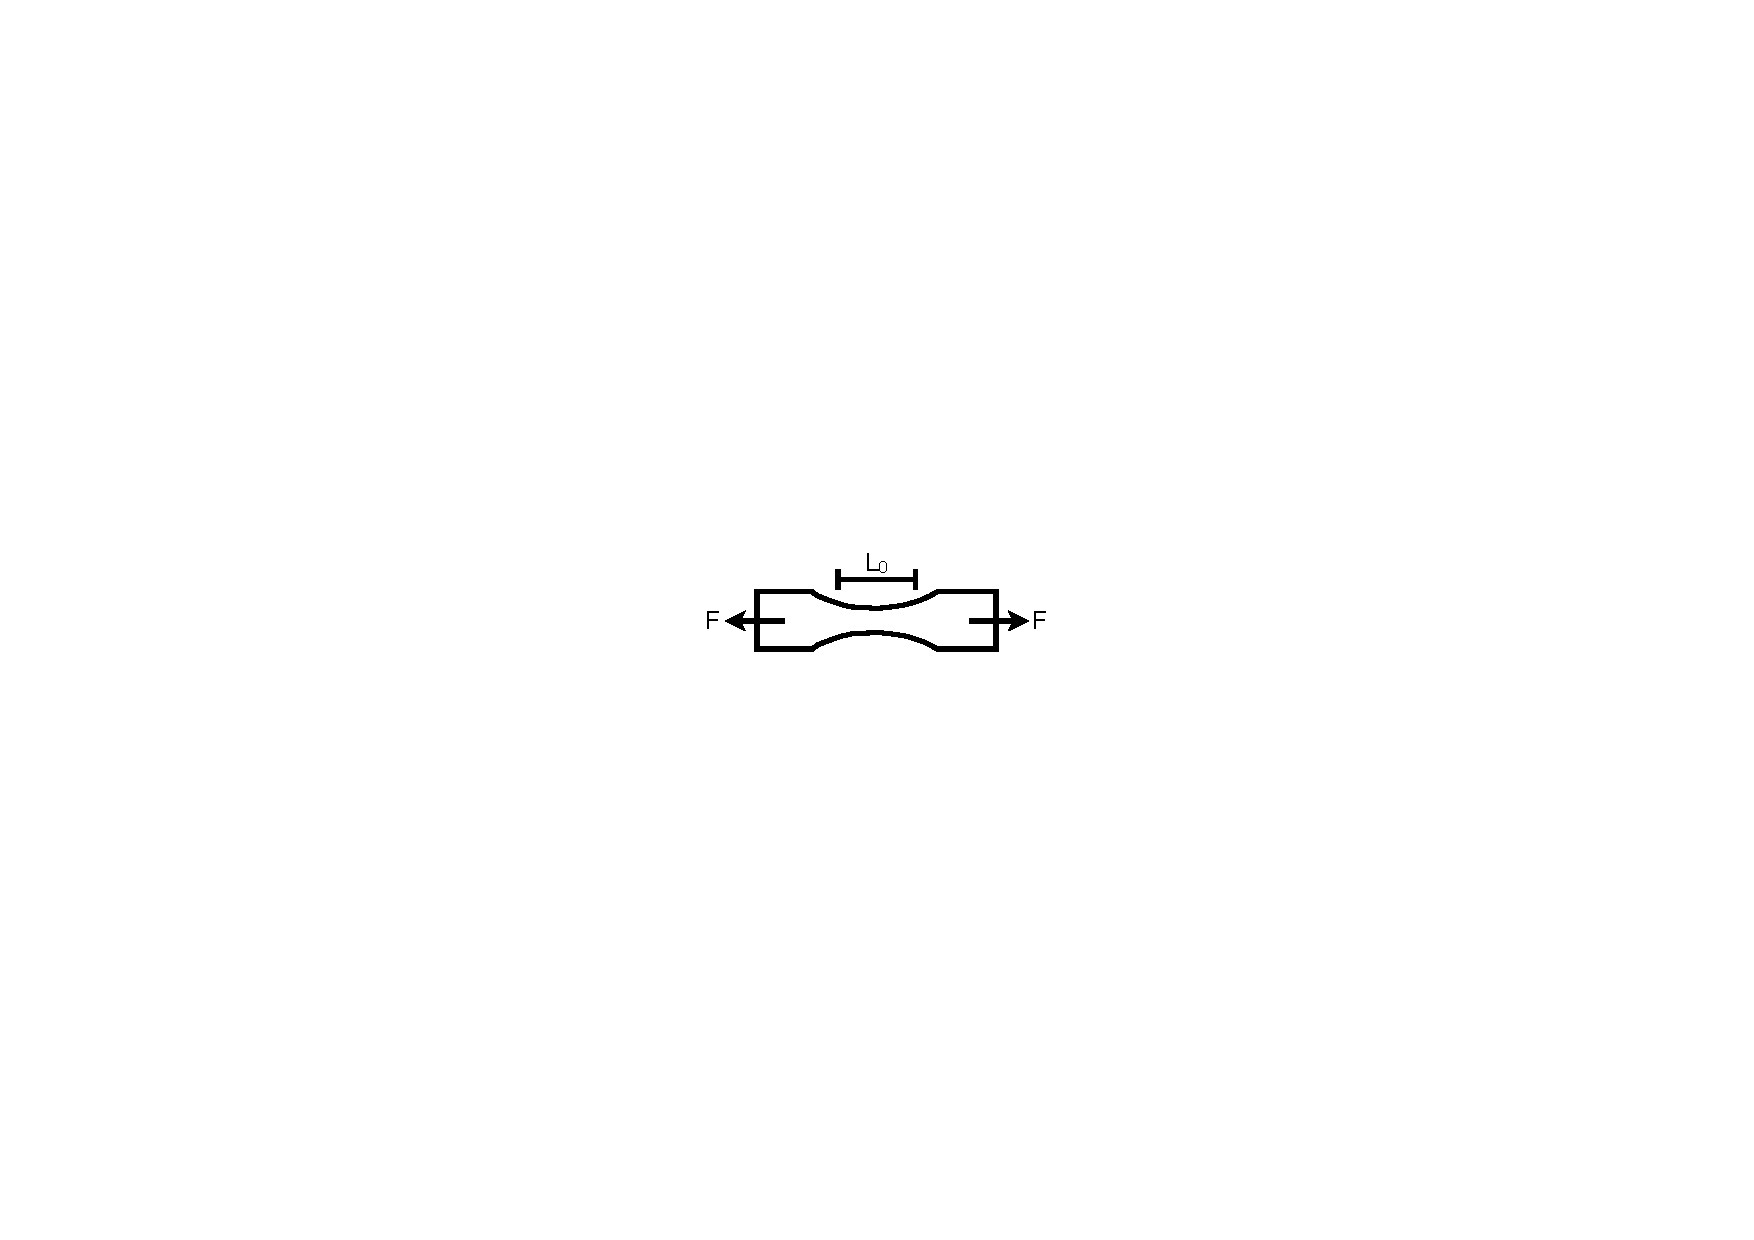
\includegraphics[width=0.45\linewidth]{Graphics/Additional-Ex/tension-test}
	\caption{Tension test specimen}
	\label{fig:tension-test}
\end{figure}
During the test, the force $F$ needed to pull the specimen and the length $L$ of a gauge section are measured. This data is used for plotting a stress-strain diagram of the material. Two definitions, engineering and true, exist for stress and strain. The engineering stress $\sigma_e$ and strain $\epsilon_e$ are defined by:
\begin{equation*}
\sigma_e = \frac{F}{A_0} \quad \textrm{and} \quad  \epsilon_e = \frac{L-L_0}{L_0},
\end{equation*}
where $L_0$ and $A_0$ are the initial gauge length and the initial cross-sectional area of the specimen, respectively. The true stress $\sigma_t$ and strain $\epsilon_t$ are defined by:
\begin{equation*}
\sigma_t = \frac{F}{A_0} \frac{L}{L_0} \quad \textrm{and} \quad \epsilon_t = ln \left( \frac{L}{L_0} \right)
\end{equation*}
In Table~\ref{tab:tension} are measurements of force and gauge length from a tension test with an aluminium specimen. The specimen has a round cross section with a radius of 6.4~mm (before the test). The initial gauge length is $L_0 = 25~mm$. Use the data to calculate and plot the engineering and true stress-strain curves, both on the same plot, of the material.
\begin{table}[h]
	\caption{Results of a tension test on an aluminium specimen}
	\label{tab:tension}
	\myfloatalign
	\begin{tabular}{lcccccccc}\toprule
	\spacedlowsmallcaps{Force (N)} & 0 & 13345 & 26689 & 40479 & 42703 & 43592 & 44482 & 44927 \\
	\spacedlowsmallcaps{Length (mm)} & 25 & 25.037 & 25.073 & 25.113 & 25.122 & 25.125 & 25.132 & 25.144 \\ \midrule
	\spacedlowsmallcaps{Force (N)} & 45372 & 46276 & 47908 & 49035 & 50265 & 53213 & 56161 & \\
	\spacedlowsmallcaps{Length (mm)} & 25.164 & 25.208 & 25.409 & 25.646 & 26.084 & 27.398 & 29.250 & \\ 
	\bottomrule
	\end{tabular}
\end{table}

\newpage
\item \textit{2D plotting}\\
A resistor, $R=4~\Omega$, and an inductor, $L=1.3~H$, are connected in a circuit to a voltage source as shown in Figure~\ref{fig:RL-circuit}a. 
\begin{figure}[h]
	\myfloatalign
	\subfloat[Circuit layout]
    {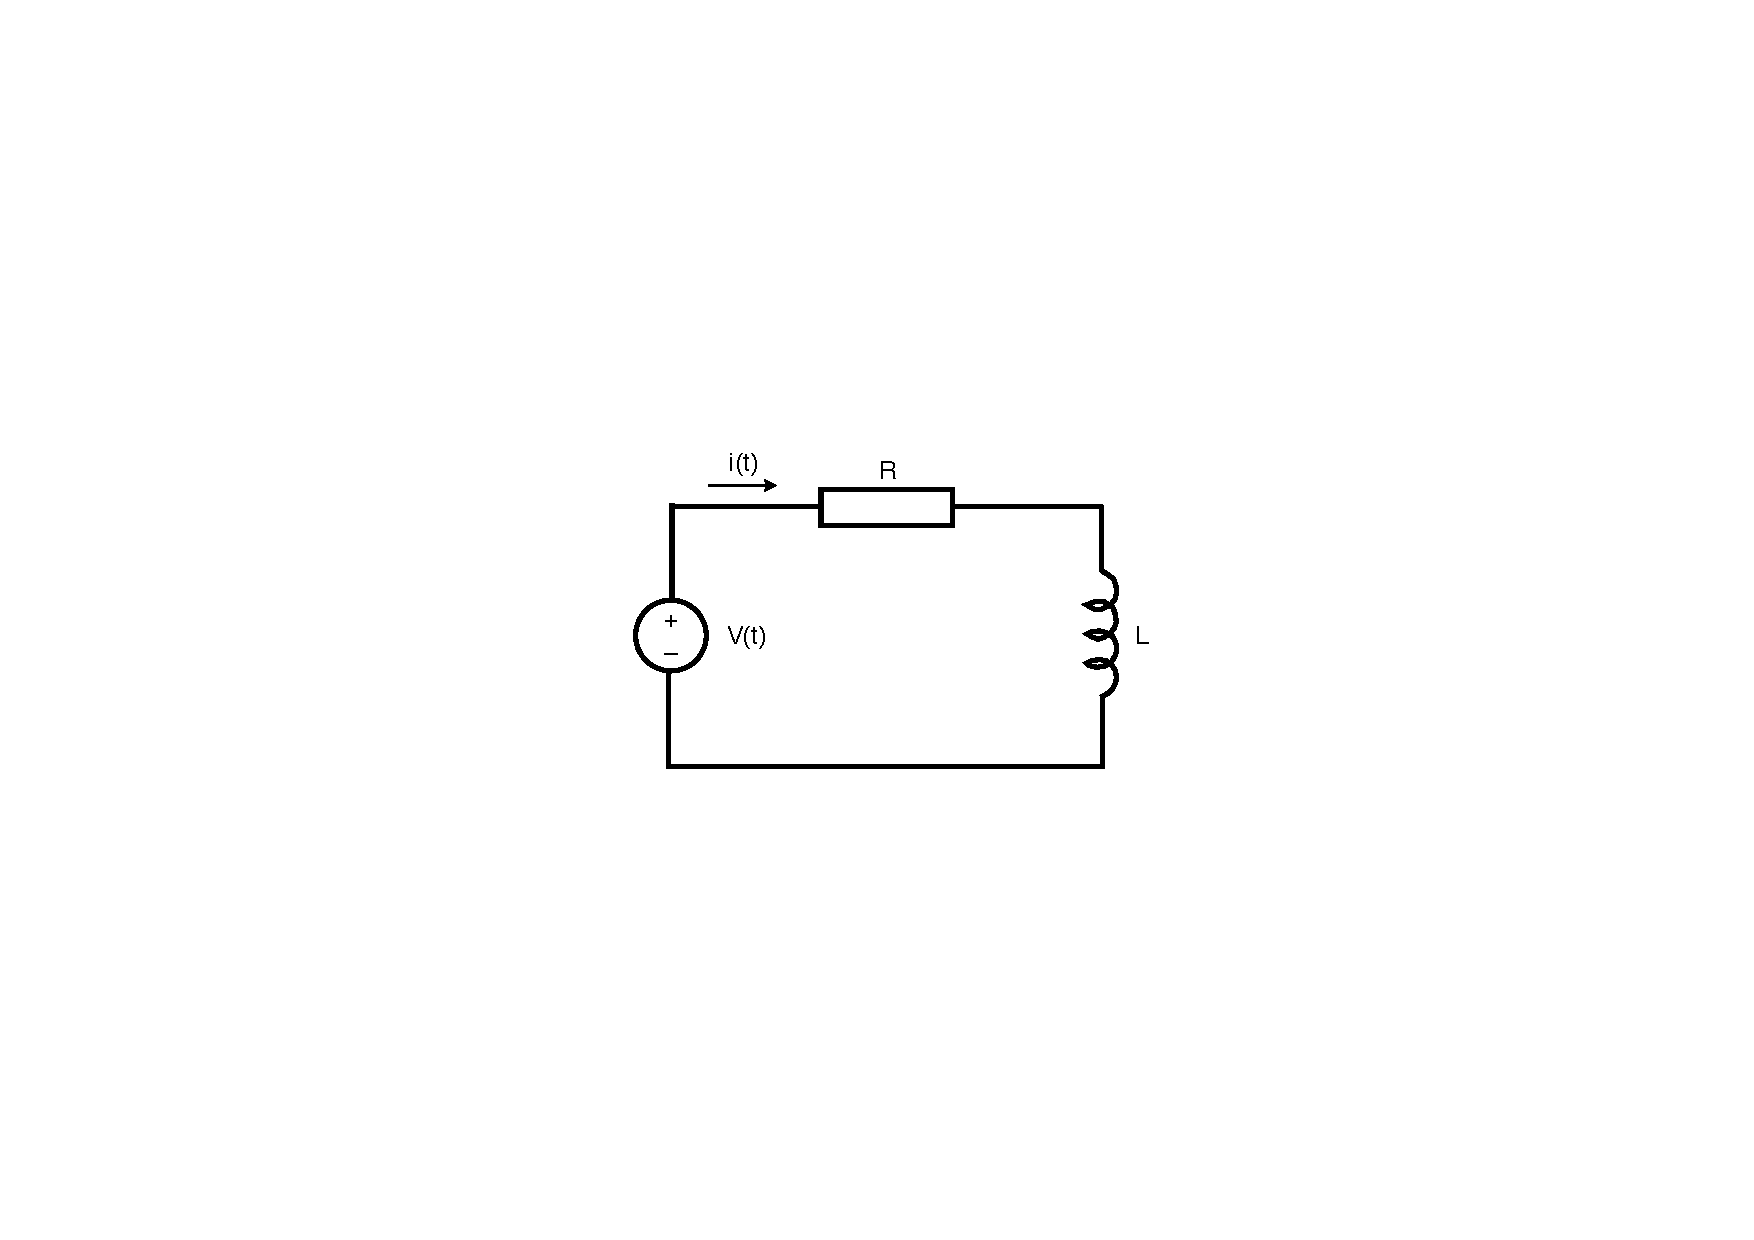
\includegraphics[width=0.45\linewidth]{Graphics/Additional-Ex/RL-circuit}}
    \subfloat[Voltage input]
    {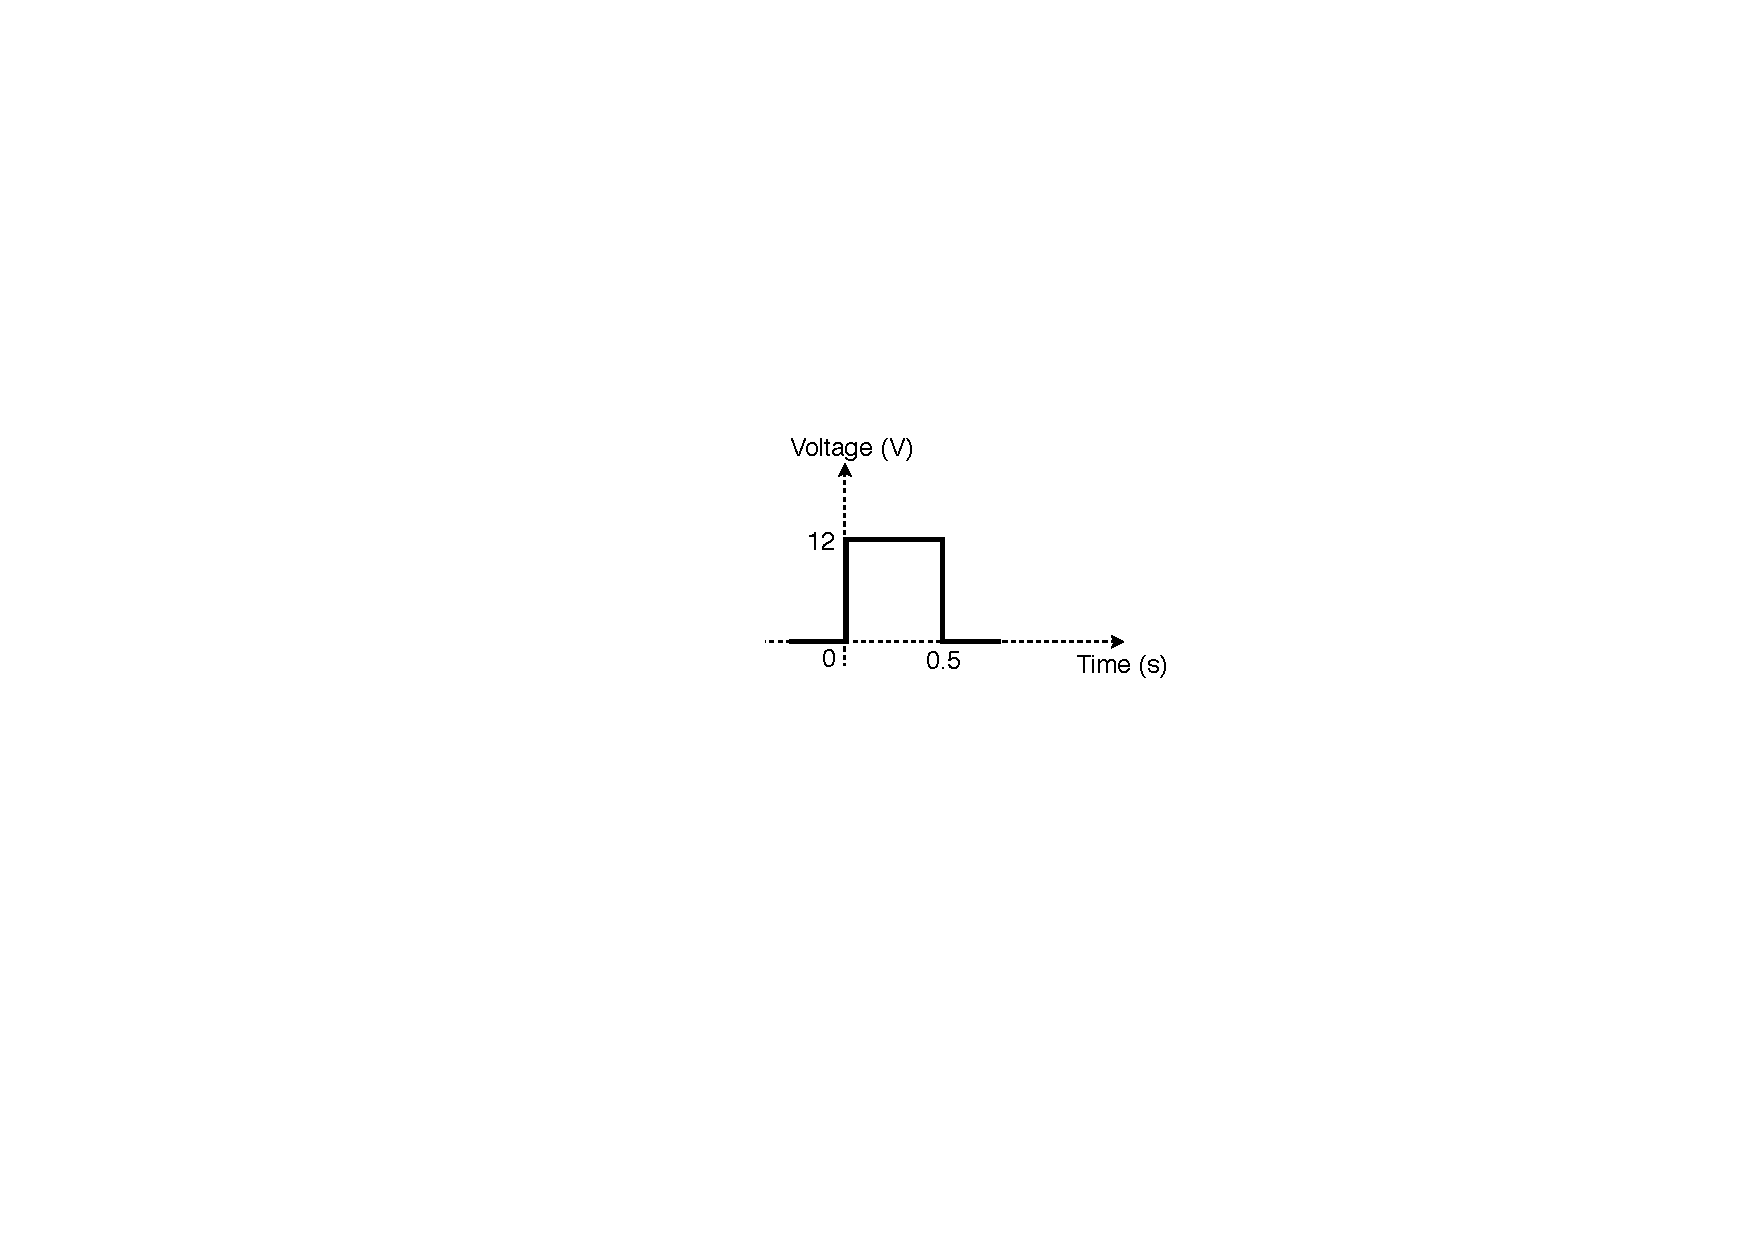
\includegraphics[width=0.45\linewidth]{Graphics/Additional-Ex/RL-circuit-ip}}
    \caption{\textit{RL} circuit}
	\label{fig:RL-circuit}
\end{figure}
When the voltage source applies a rectangular pulse with an amplitude of $V=12~V$ and a duration of $0.5~s$, as shown in Figure~\ref{fig:RL-circuit}b, the current $i(t)$ in the circuit as a function of time is given by:
\begin{align*}
i(t) &= \frac{V}{R} \left( 1-e^{\frac{-Rt}{L}} \right) \quad \textrm{for} \quad 0 \leq t \leq 0.5~s \\
i(t) &= e^{\frac{-Rt}{L}} \frac{V}{R} \left( e^{\frac{0.5R}{L}} -1 \right) \quad \textrm{for} \quad 0.5 \leq t~s
\end{align*}
Make a plot of the current as a function of time for $0\leq t \leq 2~s$.

\newpage
\item \textit{2D plotting}\\
The vibrations of a helicopter due to the periodic force applied by the rotation of the rotor can be modelled by a frictionless spring-mass-damper system subjected to an external periodic force as shown in Figure~\ref{fig:heli-vib}. 
\begin{figure}[h]
	\myfloatalign
	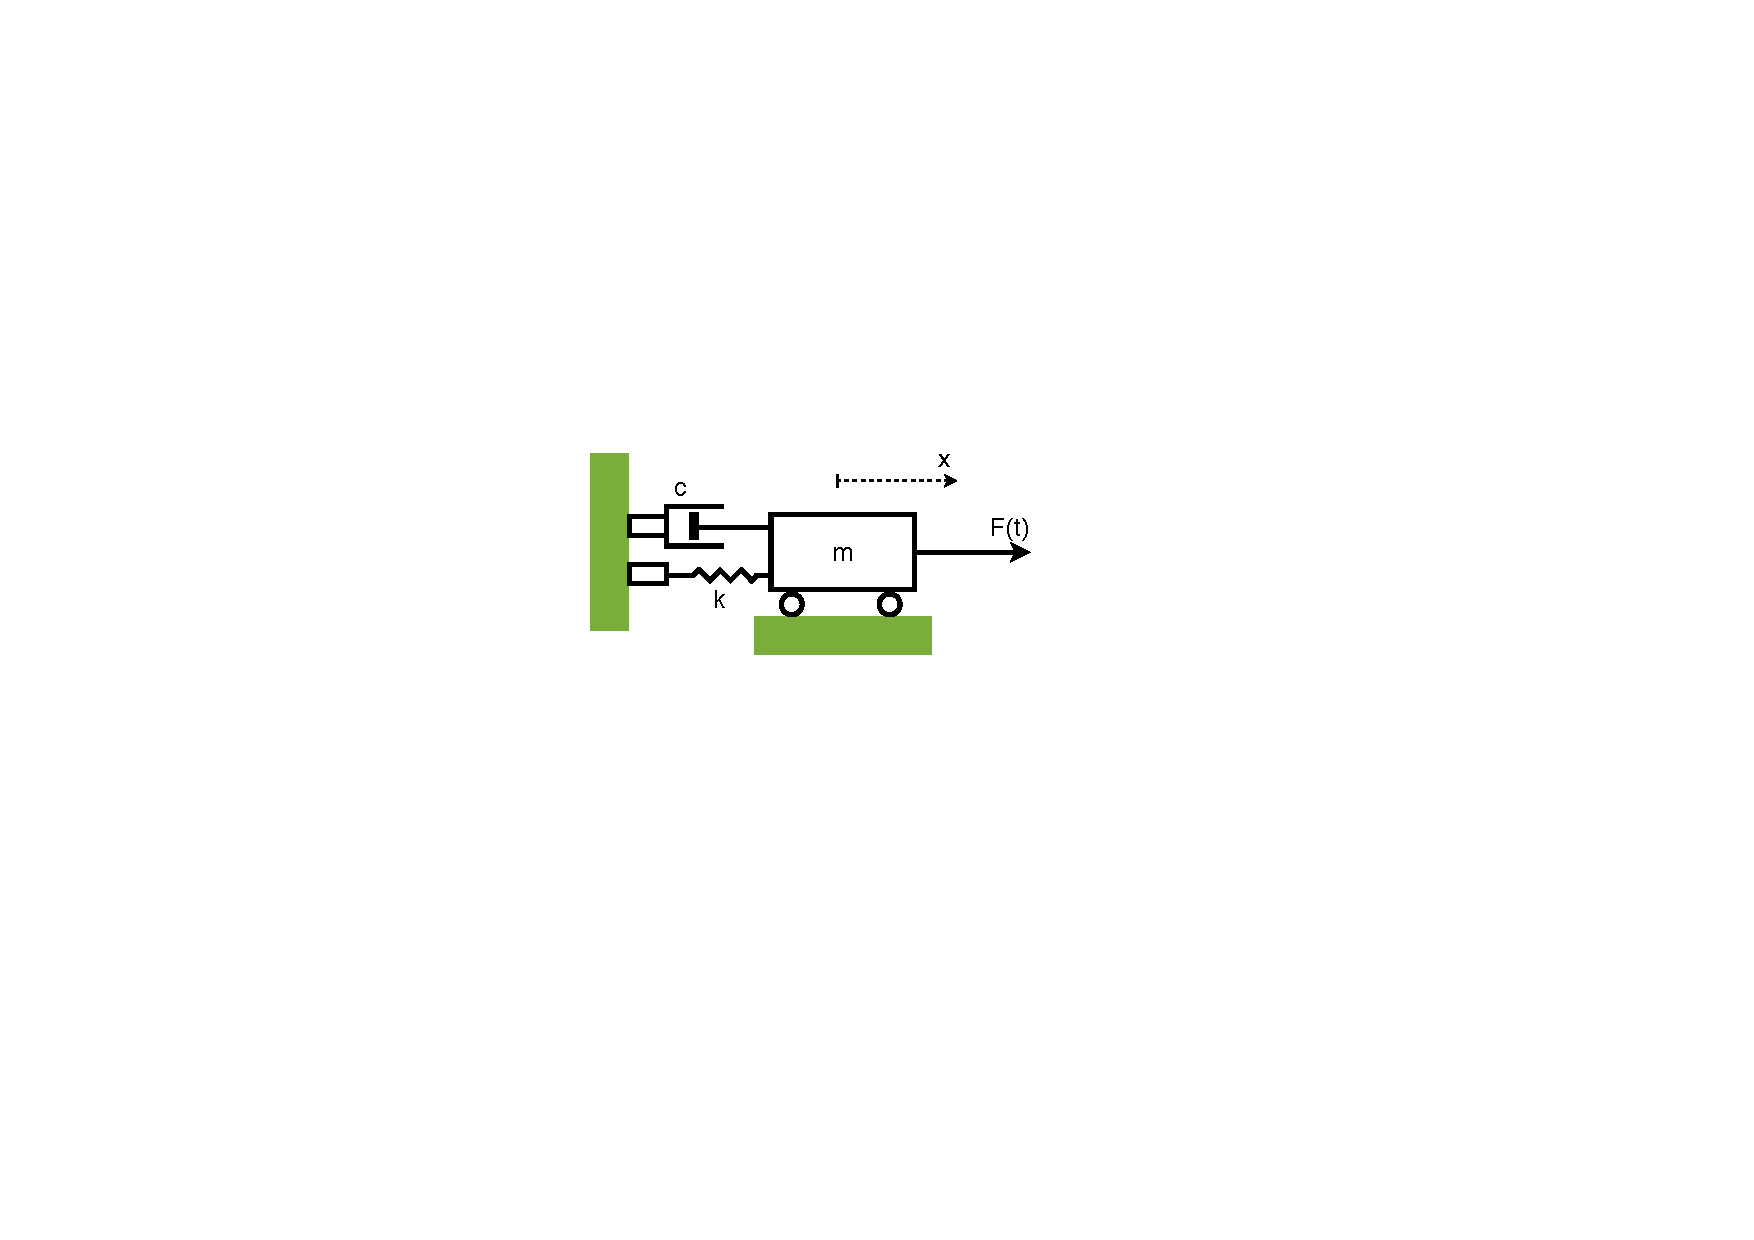
\includegraphics[width=0.55\linewidth]{Graphics/Additional-Ex/heli-vib}
	\caption{Modelling helicopter rotor vibrations with spring-mass-damper system}
	\label{fig:heli-vib}
\end{figure}
The position $x(t)$ of the mass is given by the equation:
\begin{equation*}
x(t) = \frac{2f_0}{{\omega_n}^2 - \omega_2} \sin \left( \frac{\omega_n - \omega}{2} t \right) \sin \left( \frac{\omega_n - \omega}{2} t \right),
\end{equation*}
where $F(t) = F_0 \sin(\omega t)$, and $f_0 = \frac{F_0}{m}$, $\omega$ is the frequency of the applied force, and $\omega_n$ is the natural frequency of the helicopter. When the value of $\omega$ is close to the value of $\omega_n$ the vibration consists of fast oscillation with slowly changing amplitude called beat. Use $\frac{F_0}{m} = 12~N/kg$, $\omega_n = 10~rad/s$, and $\omega = 12~rad/s$ to plot $x(t)$ as a function of t for $0\leq t\leq 10~s$.

\item \textit{2D plotting}\\
The ideal gas equation states that $\frac{PV}{RT} = n$, where $P$ is the pressure, $V$ is the volume, $T$ is the temperature, $R = 0.08206~(L~atm)/(mole~K)$ is the gas constant, and $n$ is the number of moles. For one mole ($n=1$) the quantity $\frac{PV}{RT}$ is a constant equal to 1 at all pressures. Real gases, especially at high pressures, deviate from this behaviour. Their response can be modelled with the van der Waals equation:
\begin{equation*}
P = \frac{nRT}{V-nb} - \frac{n^2a}{V^2},
\end{equation*}
where $a$ and $b$ are material constants. Consider 1~mole ($n=1$) of nitrogen gas at $T=300~K$ ($a=1.39~L^2atm/mole^2$, and $b=0.0391~L/mole$). Use the van der Waals equation to calculate $P$ as a function of $V$ for $0.08\leq V \leq 6~L$, using increments of $0.02~L$. At each value of $V$ calculate the value of $\frac{PV}{RT}$ and make a plot of $\frac{PV}{RT}$ versus $P$. Does the response of nitrogen agree with the ideal gas equation?

\item \textit{2D plotting}\\
A simply supported beam that is subjected to a constant distributed load $w$ over two-thirds of its length is shown in Figure~\ref{fig:steel-beam}. 
\begin{figure}[h]
	\myfloatalign
	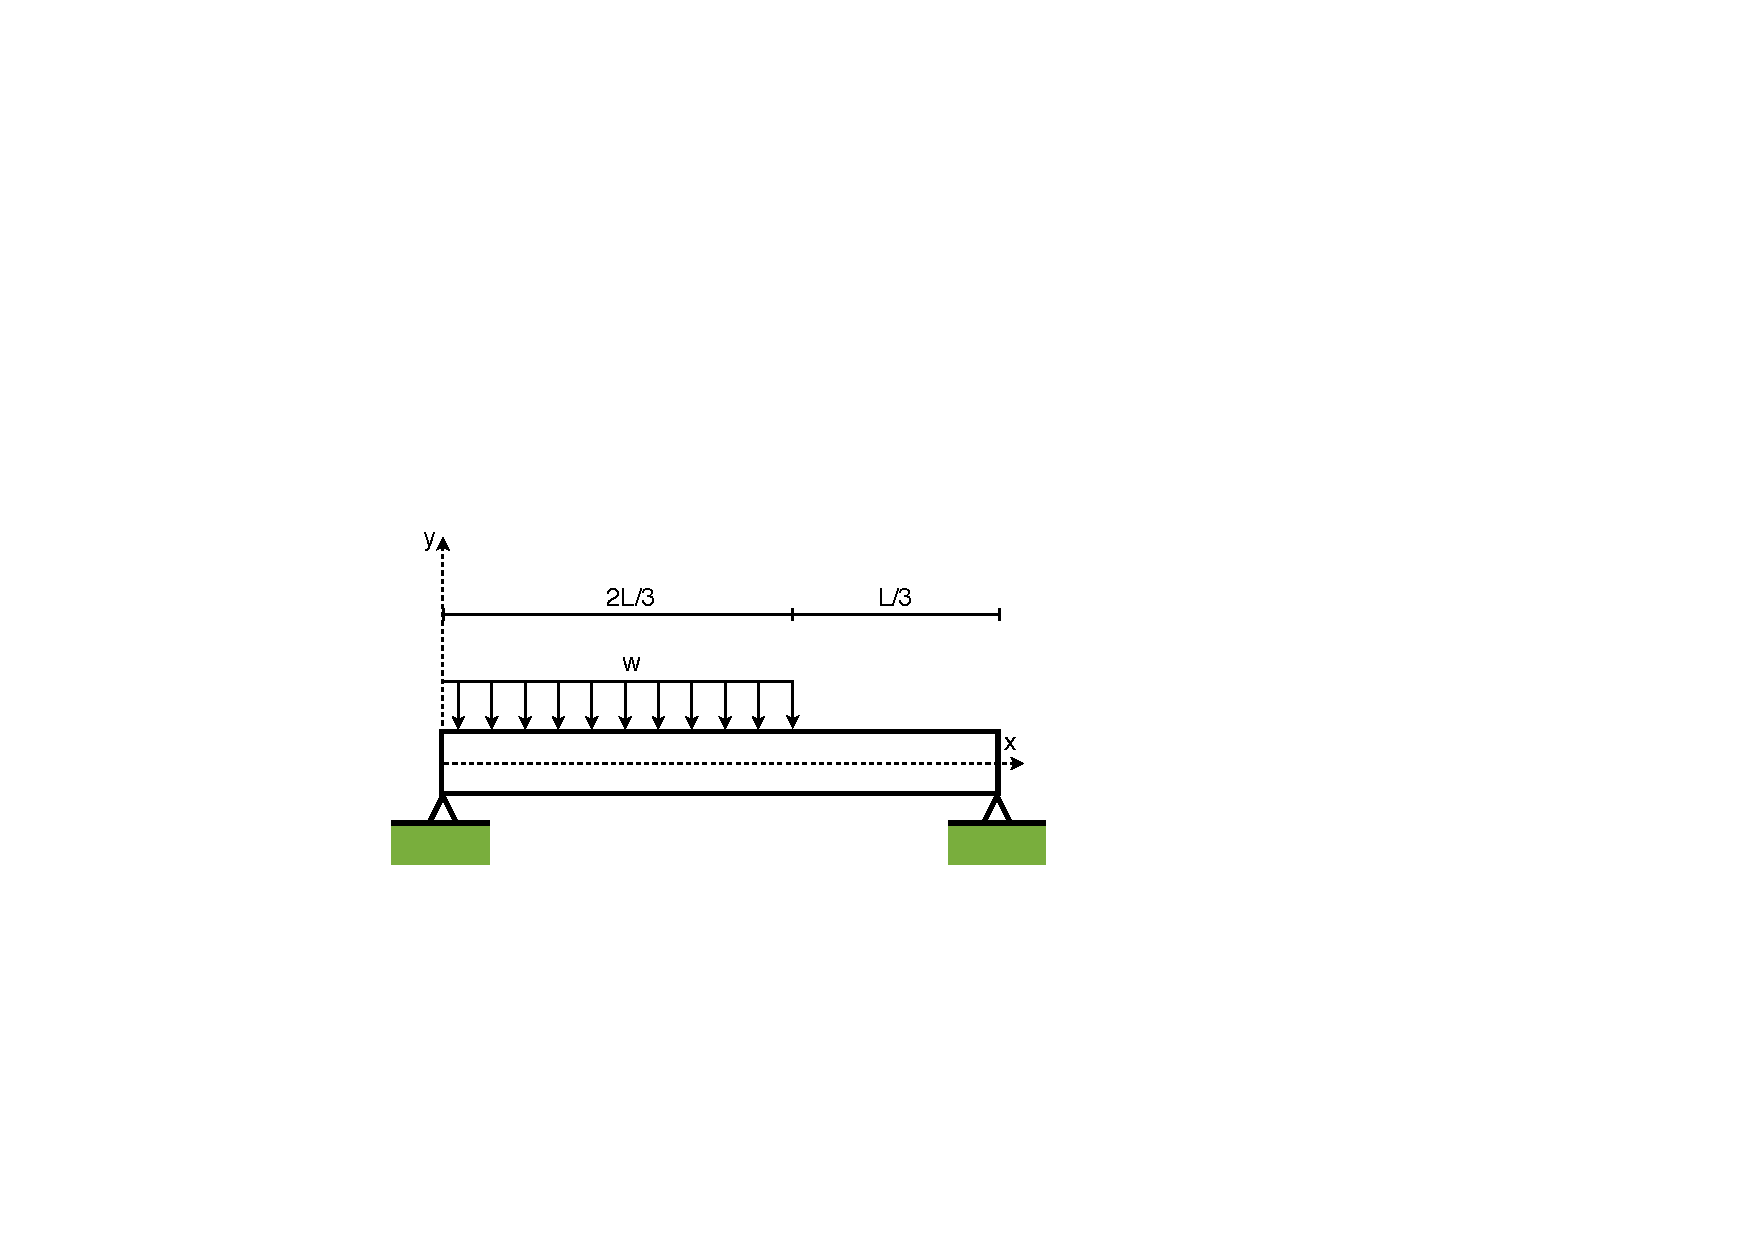
\includegraphics[width=0.75\linewidth]{Graphics/Additional-Ex/steel-beam}
	\caption{A simply supported beam}
	\label{fig:steel-beam}
\end{figure}
The deflection $y$, as a function of $x$, is given by the equations:
\begin{align*}
y &= \frac{-wx}{24LEI} \left( Lx^3 - \frac{16}{9}L^2x^2 + \frac{64}{81}L^4 \right) \quad \textrm{for} \quad 0 \leq x \leq \frac{2}{3}L, \\
y &= \frac{-wL}{54EI} \left( 2x^3 - 6Lx^2 + \frac{40}{9}L^2x - \frac{4}{9}L^3 \right) \quad \textrm{for} \quad \frac{2}{3}L \leq x \leq L,
\end{align*}
where $E$ is the elastic modulus, $I$ is the moment of inertia, and $L$ is the length of the beam. For the beam shown in Figure~\ref{fig:steel-beam}, $L=20~m$, $E=200\times 10^9~Pa$ (steel), $I=348 \times 10^{-6}~m^4$, and $w=5 \times 10^3~N/m$. Make a plot of the deflection of the beam $y$ as a function of $x$.

\item \textit{3D plotting}\\
An anti-symmetric cross-ply composite laminate has two layers where fibres are aligned perpendicular to one another. A laminate of this type will deform into a saddle shape due to residual thermal stresses as described by the equation:
\begin{equation*}
w = k(x^2-y^2),
\end{equation*}
where $x$ and $y$ are the in-plane coordinates, $w$ is the out-of-plane deflection,, and $k$ is the curvature (a complicated function of material properties and geometry). Make a \threed surface plot showing the deflection of a 100 $\times$ 100~mm square plate ($-50\leq x \leq 50$, $-50\leq y \leq 50$) assuming $k=0.254~mm^{-1}$.

\item \textit{3D plotting}\\
The van der Waals equation gives a relationship between the pressure $P (atm)$, volume $V (L)$, and temperature $T (K)$ for a real gas: 
\begin{equation*}
P = \frac{nRT}{V-nb} - \frac{n^2a}{V^2},
\end{equation*}
where $n$ is the number of moles, $R = 0.08206~(L~atm)/(mole~K)$ is the gas constant, and $a (L^2atm/mole^2)$ and $b (L/mole)$ are material constants. Consider 1.5~moles of nitrogen ($a=1.39~L^2atm/mole^2$, and $b=0.0391~L/mole$). Make a \threed surface plot that shows the variation of pressure (dependent variable, $z$ axis) with volume (independent variable, $x$ axis) and temperature (independent variable, $y$ axis). The domains for volume and temperature are: $0.3 \leq V \leq 1.2~L$ and $273 \leq T \leq 473~K$.

\item \textit{3D plotting}\\
The normal stress $\sigma_{xx}$ at point ($y,z$) in the cross section of a rectangular beam, due to the applied force $F$ at point ($y_F,z_F$) is given by:
\begin{equation*}
\sigma_{xx} = \frac{F}{A} + \frac{F~z_F~z}{I_{yy}} + \frac{F~y_F~y}{I_{zz}},
\end{equation*}
where $I_{zz}$ and $I_{yy}$ are the area moments of inertia defined by:
\begin{equation*}
I_{zz} = \frac{1}{12} bh^3 \quad \textrm{and} \quad I_{yy} = \frac{1}{12}hb^3
\end{equation*}
\begin{figure}[h]
	\myfloatalign
	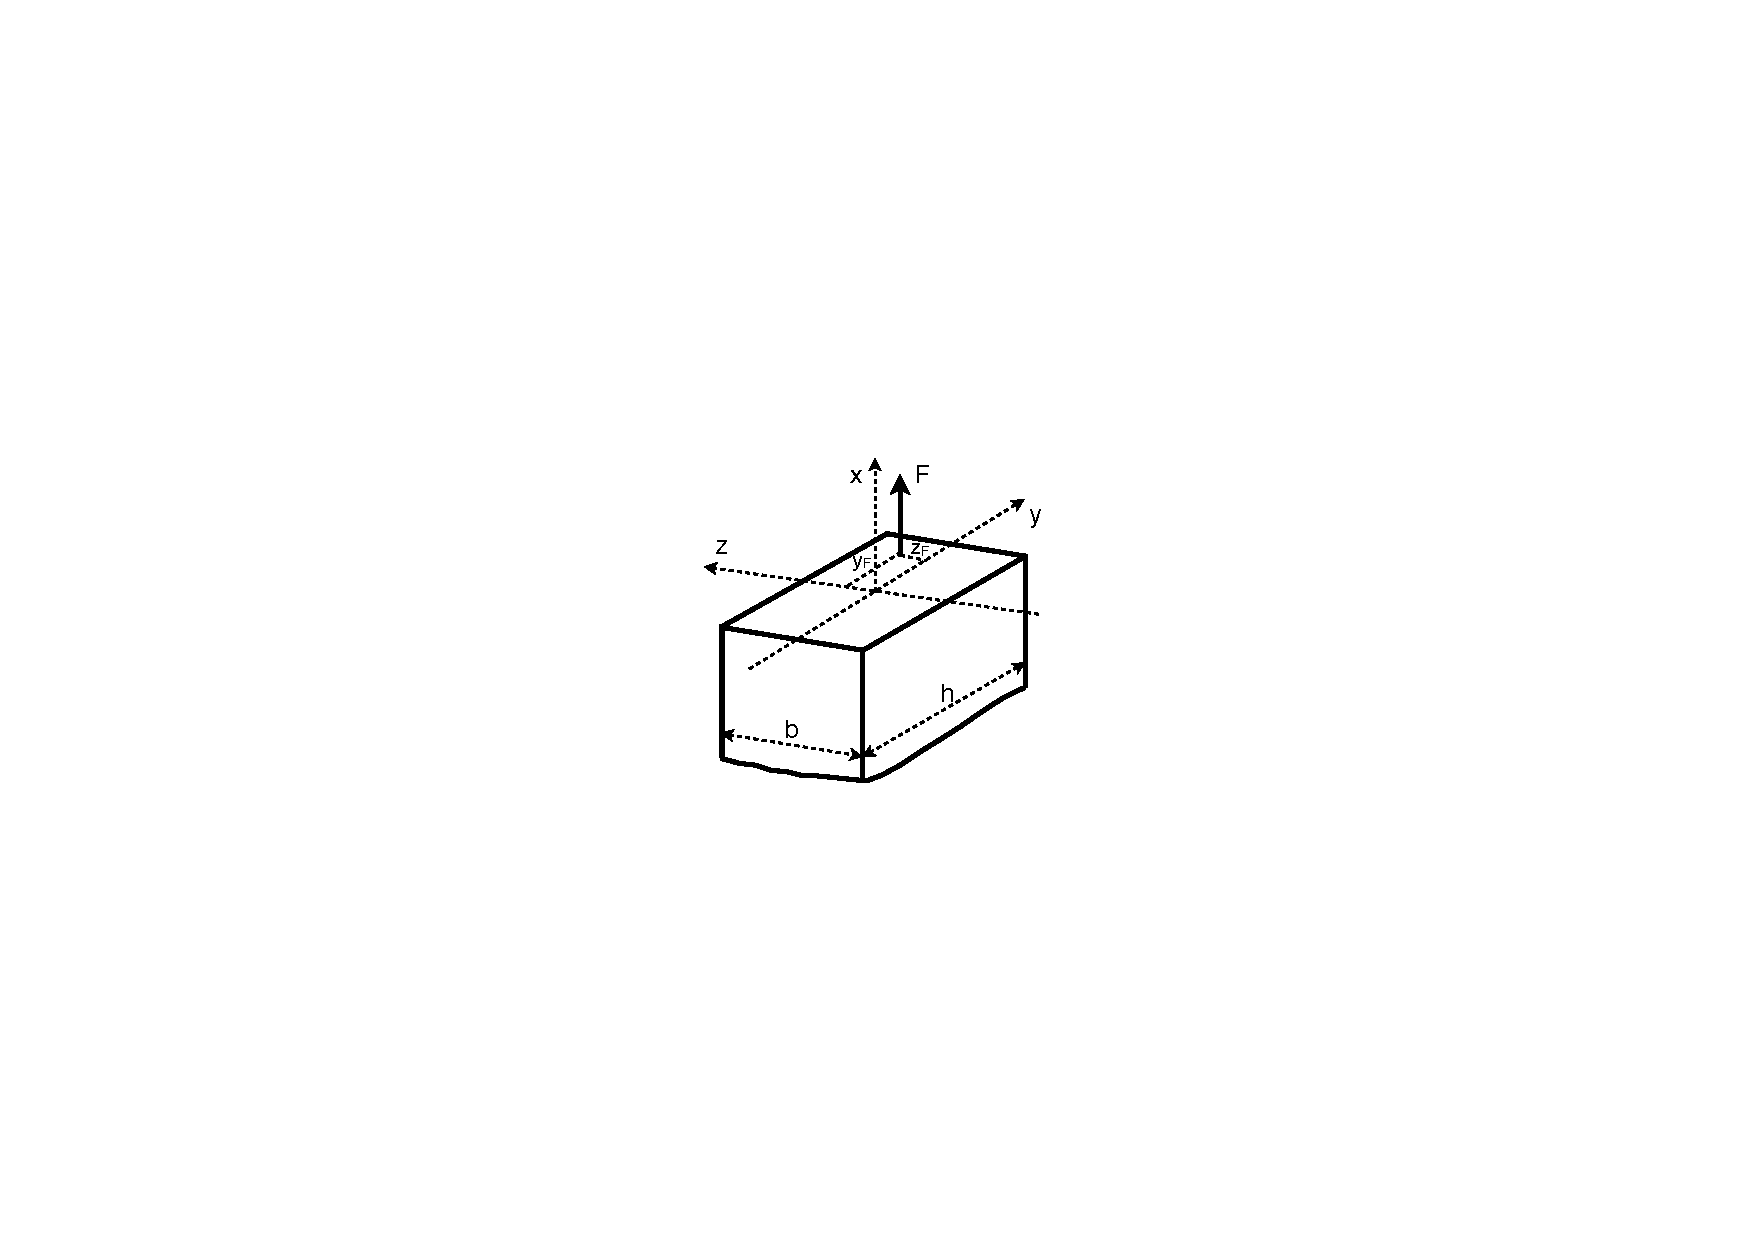
\includegraphics[width=0.45\linewidth]{Graphics/Additional-Ex/beam-stress}
	\caption{Cross section of a rectangular beam}
	\label{fig:beam-stress}
\end{figure}
Determine and make a \threed surface plot of the normal stress in the cross-sectional area shown in Figure~\ref{fig:beam-stress}, given that: $h=40~mm$, $b=30~mm$, $y_F=-15~mm$, $z_F=-10~mm$, and $F=-250000~N$. Plot the coordinates $y$ and $z$ in the horizontal plane, and the normal stress in the vertical direction.

\item \textit{3D plotting}\\
A defect in a crystal lattice where a row of atoms is missing is called an edge dislocation, as shown in Figure~\ref{fig:edge-disloc}. 
\begin{figure}[h]
	\myfloatalign
	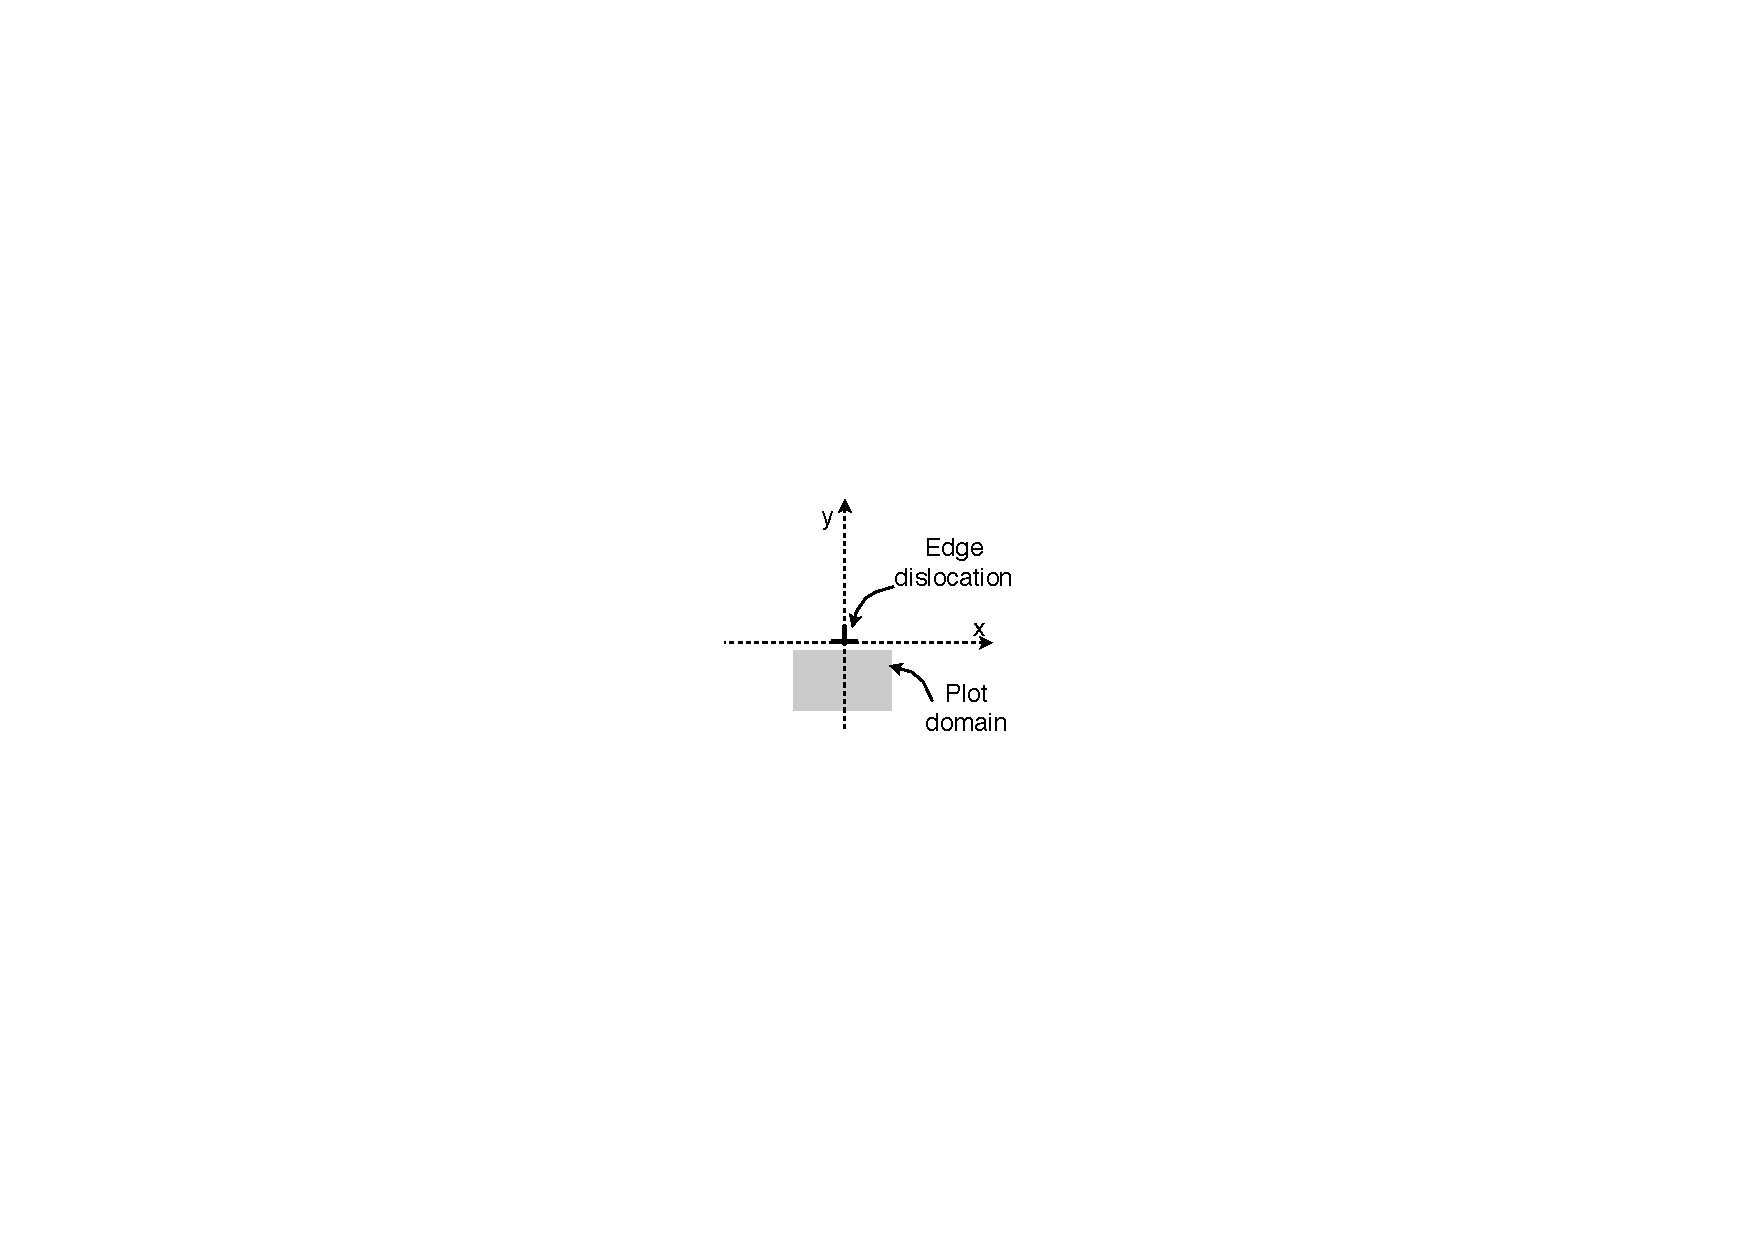
\includegraphics[width=0.4\linewidth]{Graphics/Additional-Ex/edge-disloc}
	\caption{Edge dislocation}
	\label{fig:edge-disloc}
\end{figure}
The stress field around an edge dislocation is given by:
\begin{align*}
\sigma_{xx} &= \frac{-Gby(3x^2+y^2)}{2\pi(1-\nu){(x^2+y^2)}^2}, \\
\sigma_{yy} &= \frac{Gby(x^2-y^2)}{2\pi(1-\nu){(x^2+y^2)}^2}, \\
\tau_{xy} &= \frac{Gbx(x^2-y^2)}{2\pi(1-\nu){(x^2+y^2)}^2},
\end{align*}
where $G$ is the shear modulus, $b$ is the Burgers vector, and $\nu$ is Poisson's ratio. Make \threed surface plots of the stress components (each in a separate figure window) due to an edge dislocation in aluminium for which $G=27.7\times 10^9~Pa$, $b=0.286\times 10^{-9}~m$, and $\nu = 0.334$. Plot the stresses in the domain $-5\times 10^{-9} \leq x \leq 5\times 10^{-9}~m$ and $-5\times 10^{-9} \leq y \leq -1\times 10^{-9}~m$. Plot the coordinates $x$ and $y$ in the horizontal plane, and the stresses in the vertical direction.

\item \textit{3D plotting}\\
Molecules of a gas in a container are moving around at different speeds. Maxwell's speed distribution law gives the probability distribution $P(v)$ as a function of temperature and speed:
\begin{equation*}
P(\nu) = 4\pi {\left( \frac{M}{2\pi RT} \right)}^{\frac{3}{2}} v^2 e^{\frac{-Mv^2}{2RT}},
\end{equation*}
where $M$ is the molar mass of the gas in $kg/mol$, $R=8.31~J/mol~K$ is the gas constant, $T$ is the temperature in $K$, and $v$ is the molecules speed in $m/s$. Make a \threed surface plot of $P(v)$ as a function of $v$ and $T$ for $0\leq v \leq 1000~m/s$ and $70\leq T \leq 320~K$ for oxygen (molar mass $M=0.032~kg/mol$).

\item \textit{3D plotting}\\
An \textit{RLC} circuit with an alternating voltage source is shown in Figure~\ref{fig:RLC-circuit}. 
\begin{figure}[h]
	\myfloatalign
	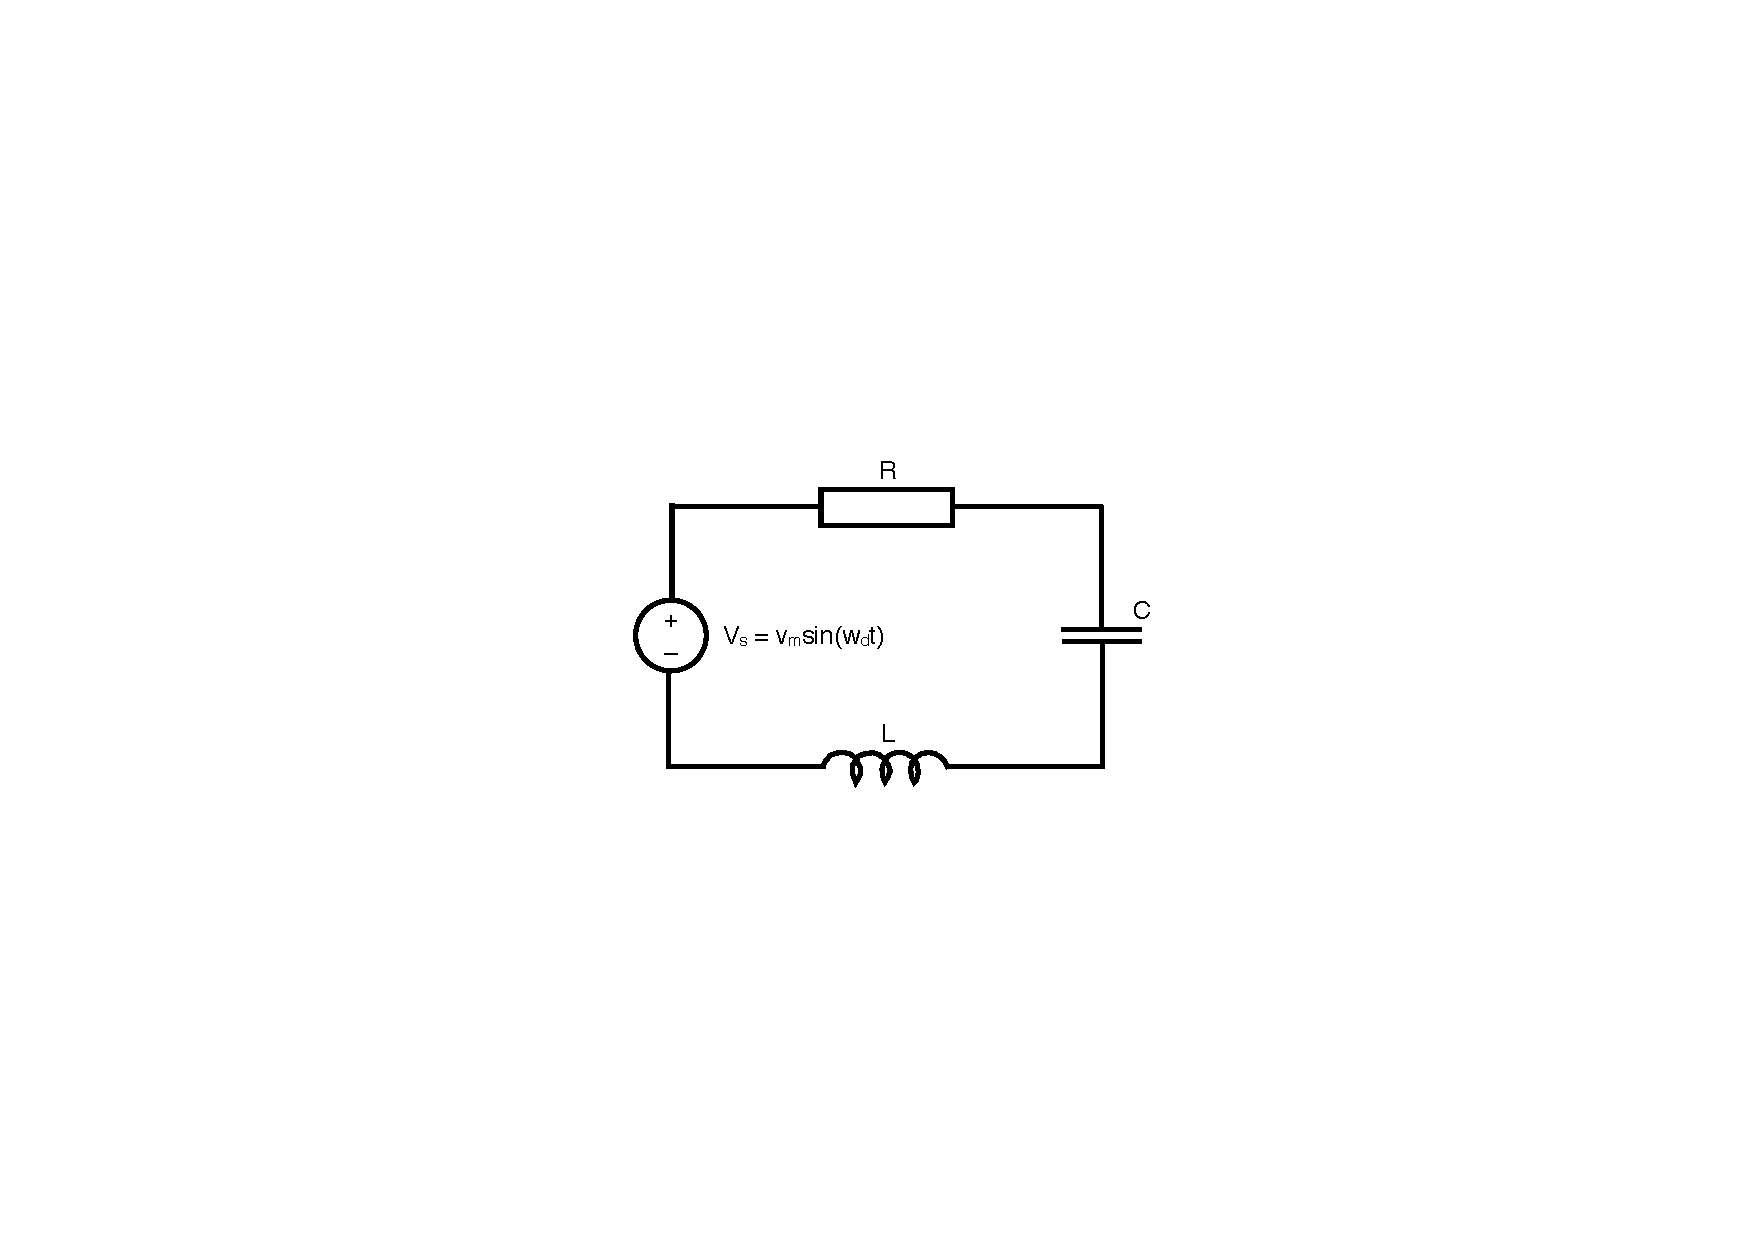
\includegraphics[width=0.65\linewidth]{Graphics/Additional-Ex/RLC-circuit}
	\caption{An \textit{RLC} circuit with an alternating voltage source}
	\label{fig:RLC-circuit}
\end{figure}
The source voltage $v_s$ is given by $v_s=v_m \sin(\omega_d t)$ where $\omega_d=2\pi f_d$ is which $f_d$ is the driving frequency. The amplitude of the current $I$ in the circuit is given by:
\begin{equation*}
I = \frac{v_m}{\sqrt{R^2 + {\left( \omega_d L - \frac{1}{\omega_d C} \right)}^2}},
\end{equation*}
where $R$ and $C$ are the resistance of the resistor and the capacitance of the capacitor, respectively. For the circuit in Figure~\ref{fig:RLC-circuit} $C=15\times 10^{-6}~F$, $L=240\times 10^{-3}~H$, and $v_m=24~V$.
\begin{enumerate}
\item Make a \threed surface plot of the current $I$ ($z$ axis) as a function of $\omega_d$ ($x$ axis) for $60\leq f \leq 110~Hz$, and a function of $R$ ($y$ axis) for $10\leq R \leq40~\Omega$.
\item Rotate the plot into the $x-z$ plane. Estimate the natural frequency of the circuit (the frequency at which $I$ is maximum). Compare the estimate with the calculated value of $1/(2\pi\sqrt{LC})$.
\end{enumerate}

\newpage
\section{Scripts and Functions} \label{sect:scripts_functions}
\item \textit{Scripts}\\
A cylindrical silo with radius $r$ has a spherical cap roof with radius $R$, as shown in Figure~\ref{fig:silo}. The height of the cylindrical portion is $H$. Write a script file that determines the height $H$ for given values or $r$, $R$, and the volume $V$. In addition the script should also calculate the surface area of the silo.
\begin{figure}[h]
	\myfloatalign
	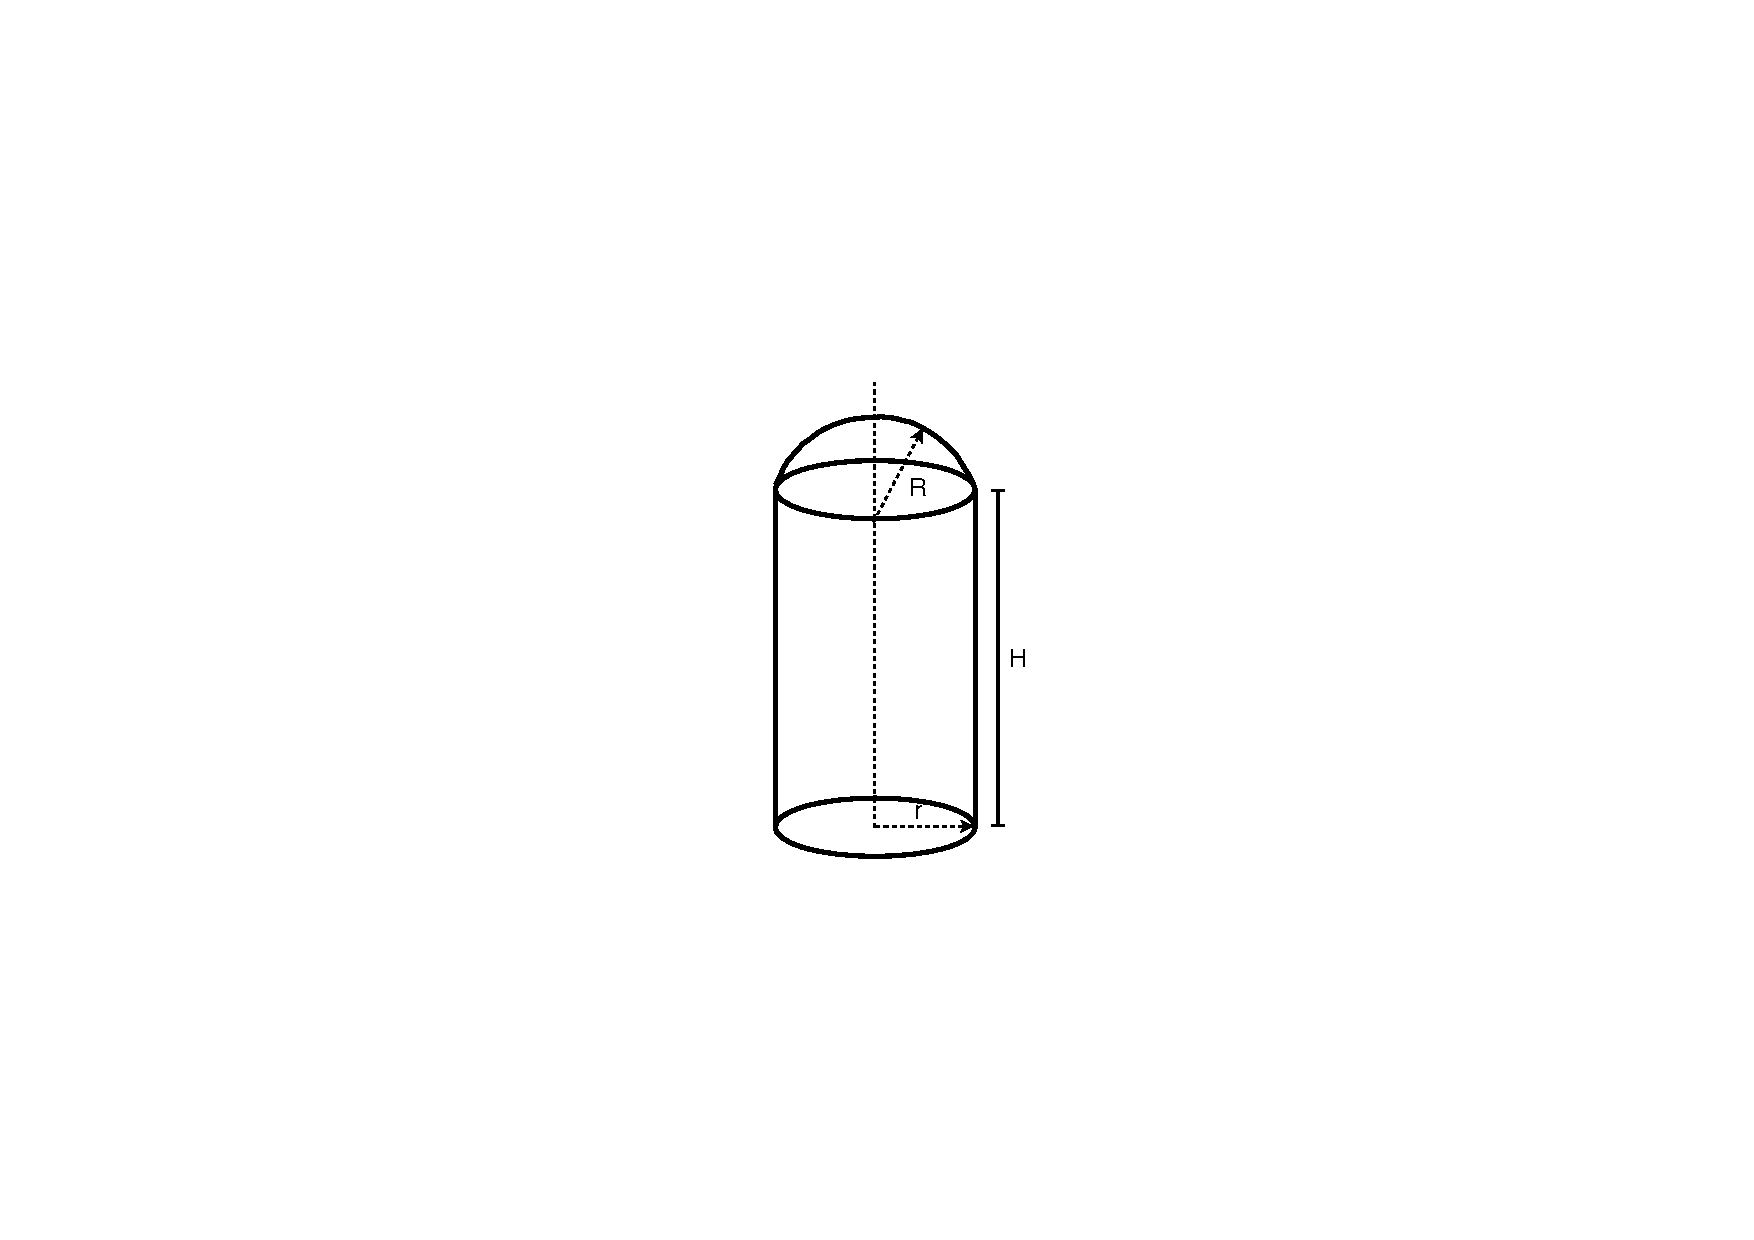
\includegraphics[width=0.35\linewidth]{Graphics/Additional-Ex/silo}\quad
	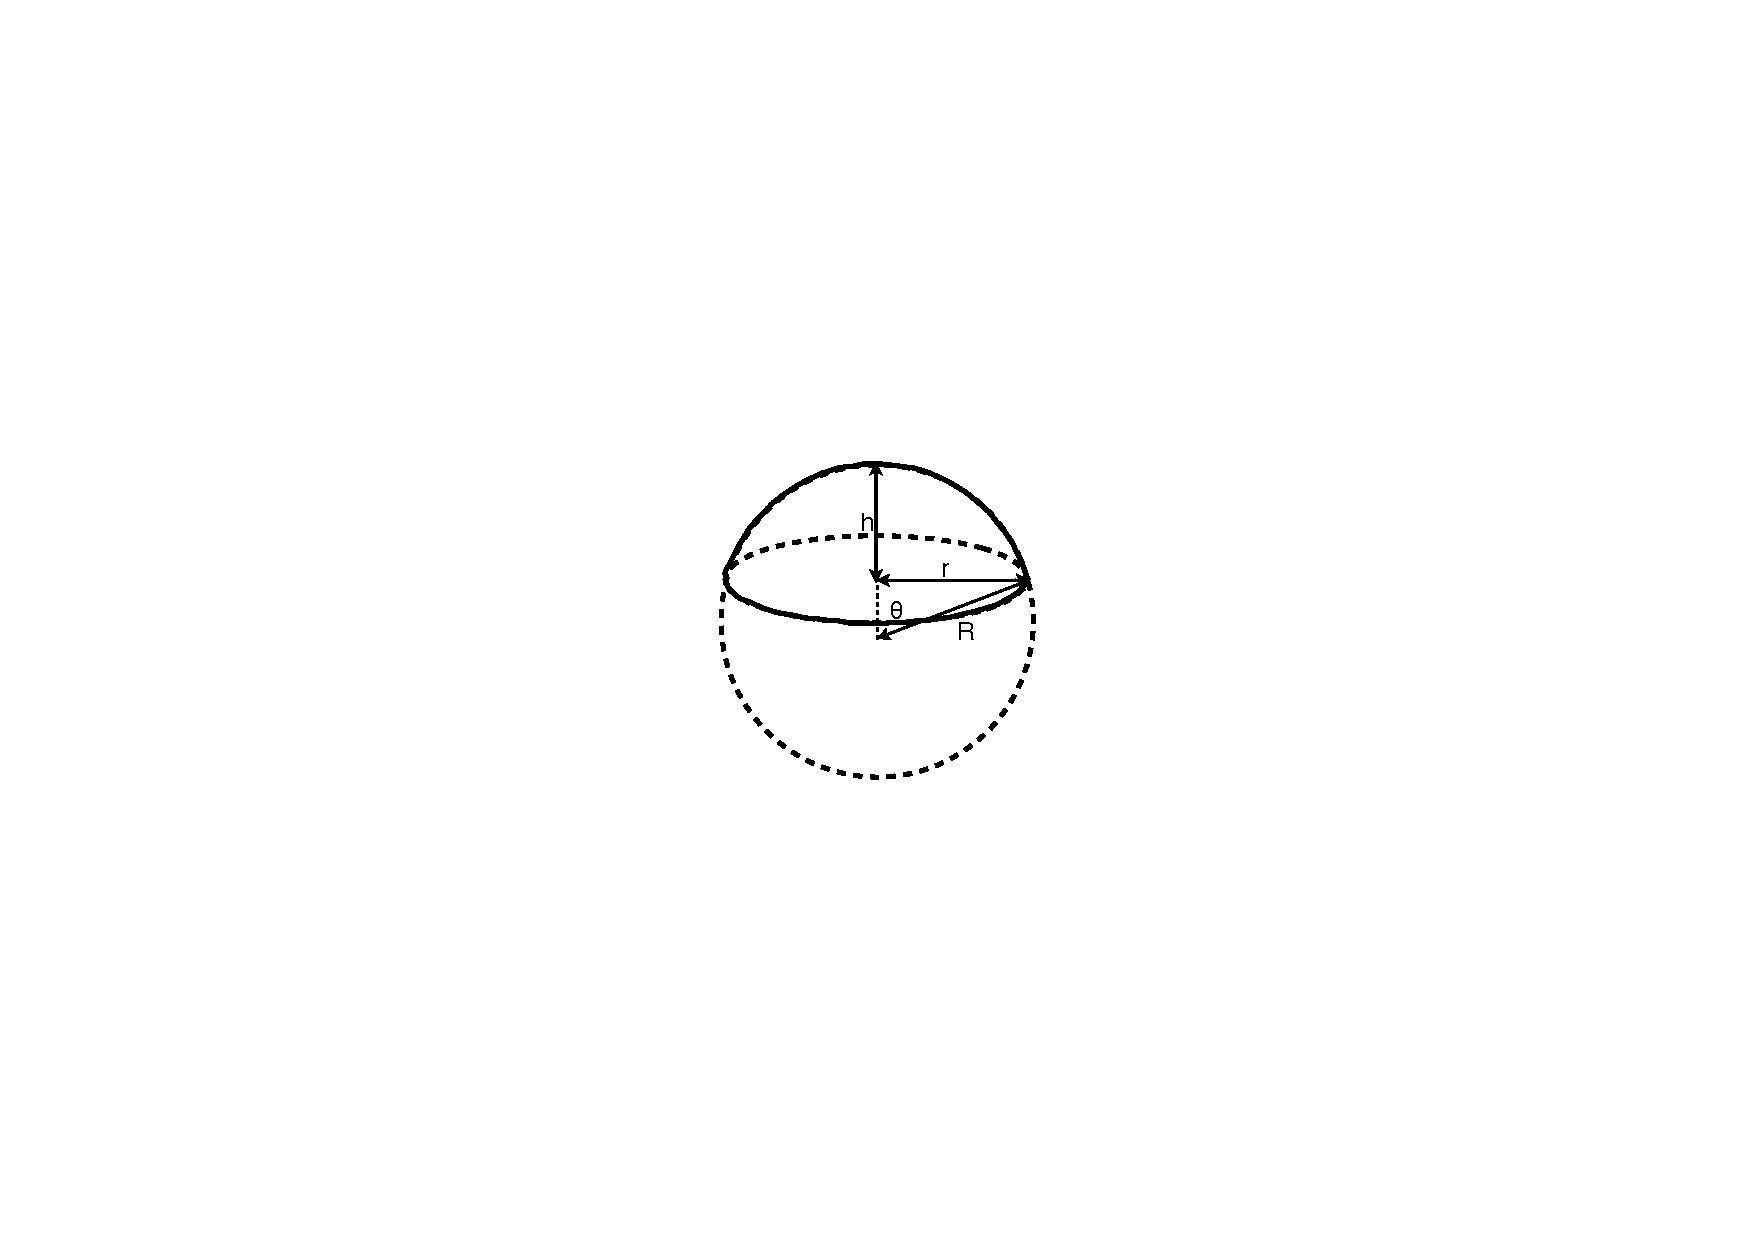
\includegraphics[width=0.35\linewidth]{Graphics/Additional-Ex/silo-cap}
	\caption{Silo}
	\label{fig:silo}
\end{figure}
The volume of the cylinder is given by:
\begin{equation*}
V_{\textrm{cyl}} = \pi r^2 H,
\end{equation*}
and the volume of the spherical cap is given by:
\begin{equation*}
V_{\textrm{cap}} = \frac{1}{3}\pi h^2 (3R-h),
\end{equation*}
where $h=R-Rcos(\theta)$ and $\theta$ is calculated from $\sin(\theta) = \frac{r}{R}$. The height $H$ of the cylindrical part can be expressed by:
\begin{equation*}
H = \frac{V-V_{\textrm{cap}}}{\pi r^2}
\end{equation*}
The surface area of the silo is obtained by adding the surface areas of the cylindrical part and the spherical cap:
\begin{equation*}
S = S_{\textrm{cyl}} + S_{\textrm{cap}} = 2\pi rH + 2\pi Rh
\end{equation*}
Calculate the height and surface area of a silo with $r=10~m$, $R=15~m$ and $V=3500~m^3$. 

\item \textit{Scripts}\\
Radioactive decay of radioactive materials can be modelled by the equation $A=A_0e^{kt}$, where $A$ is the population at time $t$, $A_0$ is the amount at $t=0$, and $k$ is the decay constant ($k\leq 0$). Technetium-99 is a radioisotope that is used in the imaging of the brain. Its half-life time is 6~hours. Write a script to calculate the relative amount of Technetium-99 ($A/A_0$) in a patient body for 24~hours after receiving a dose. After determining the value of $k$, define a vector \mcode{t=0:2:24} and then calculate and plot the corresponding values of $A/A_0$.

\item \textit{Scripts}\\
The variation of vapour pressure $P$ (in units of mm Hg) of benzene with temperatures (in $^\circ C$) in the range $8^\circ C \leq T \leq 80^\circ C$ can be modelled with the Antoine equation\graffito{Constants for the Antoine equation taken from the \href{http://www.ddbst.com/en/online/Online_Calc_vap_Form.php}{Dortmund Data Base}.}:
\begin{equation*}
log_{10}P=A - \frac{B}{C+T}
\end{equation*}
For benzene, the values of the constants are as follows: $A = 6.87987$, $B = 1196.76$, $C = 219.161$. Write a script that calculates the vapour pressure for various temperatures. The script should create a vector of temperatures from $T = 8^\circ C$ to $T = 42^\circ C$ in increments of 2 degrees, and display a two-column table of $P$ and $T$ where the first column is temperatures in $^\circ C$, and the second column is the corresponding pressures in mm Hg. The script should also plot $P$ against $T$ and use a logarithmic axis for $P$.

\item \textit{Scripts}\\
The temperature dependance of the heat capacity $C_p$ of many gases can be described in terms of a cubic equation:
\begin{equation*}
C_p=a+bT+cT^2+dT^3
\end{equation*}
The following table gives the coefficients of the cubic equation for four gases. $C_p$ is in $Joules/(g~mol)(^\circ C)$ and $T$ is in $^\circ C$.
\begin{table}[h]
	\caption{Coefficients for the cubic equation for the heat capacity of gases}
	\label{tab:heat-cap}
	\myfloatalign
	\begin{tabular}{lcccc}\toprule
	\spacedlowsmallcaps{Gas} & $a$ & $b$ & $c$ & $d$ \\ \midrule
	$SO_2$ & $38.91$ & $3.904\times 10^{-2}$ & $-3.205\times 10^{-5}$ & $8.606\times 10^{-9}$ \\
	$SO_3$ & $48.50$ & $9.188\times 10^{-2}$ & $-8.540\times 10^{-5}$ & $32.40\times 10^{-9}$ \\
	$O_2$ & $29.10$ & $1.158\times 10^{-2}$ & $-0.6076\times 10^{-5}$ & $1.311\times 10^{-9}$ \\
	$N_2$ & $29.00$ & $0.220\times 10^{-2}$ & $-0.5723\times 10^{-5}$ & $-2.871\times 10^{-9}$ \\
	\bottomrule
	\end{tabular}
\end{table}
Write a script to calculate the heat capacity for each gas at temperatures ranging between 200 and 400$^\circ C$ at 20$^\circ C$ increments. To present the results, create an 11$\times$5 matrix where the first column is the temperature, and second to fifth columns are the heat capacities of $SO_2$, $SO_3$, $O_2$, and $N_2$, respectively.

\newpage
\item \textit{Functions}\\
Create a function file that calculates the trajectory of a projectile. The inputs to the function should be the initial velocity and the angle at which the projectile is fired. The outputs from the function should be the maximum height and distance. In addition, the function should generate a plot of the trajectory. Use the function to calculate the trajectory of a projectile that is fired at a velocity of $230~m/s$ at an angle of $39~^\circ$.
\begin{figure}[h]
	\myfloatalign
	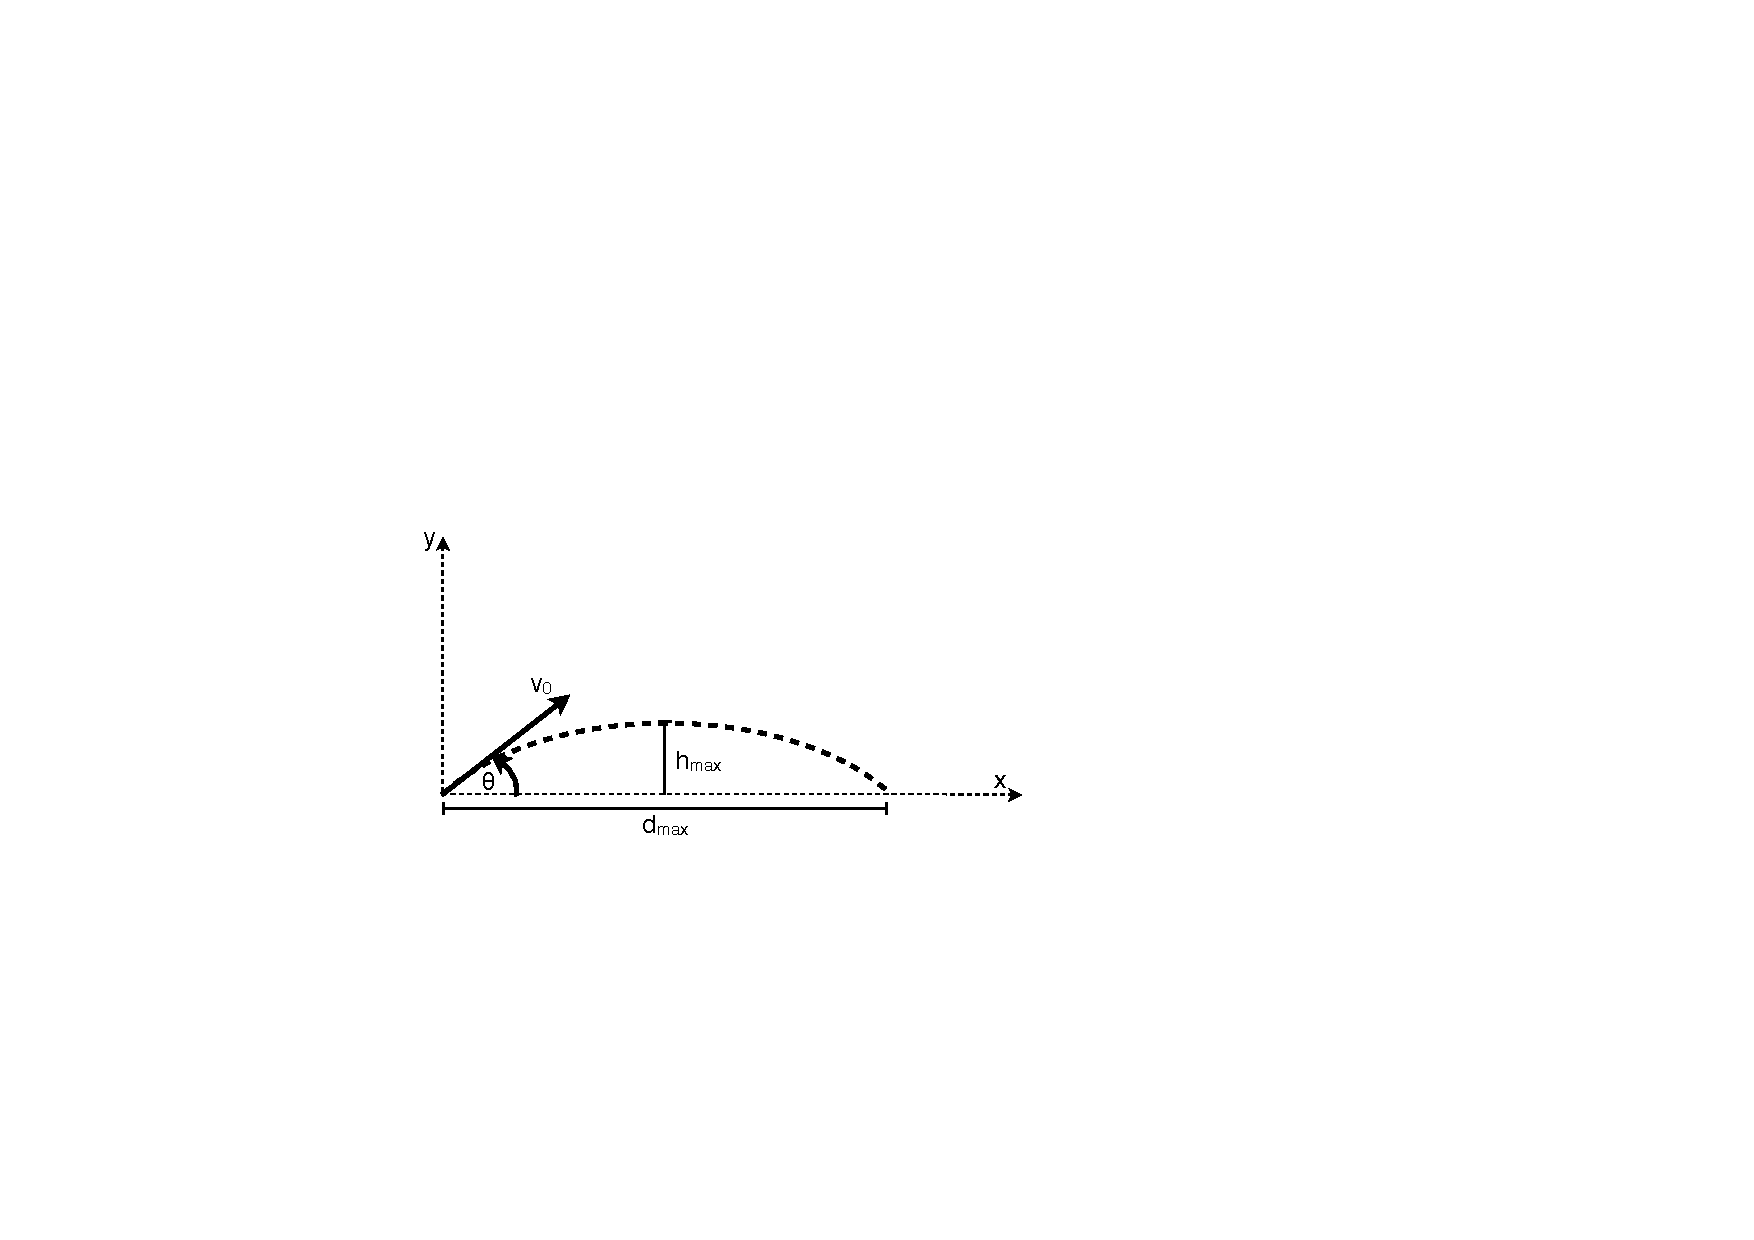
\includegraphics[width=0.75\linewidth]{Graphics/Additional-Ex/projectile}
	\caption{Motion of a projectile}
	\label{fig:projectile}
\end{figure}

\addtolength{\parindent}{-4mm}
\fcolorbox{myborderblue}{myblue}{%
\begin{minipage}{\linewidth}
\begin{minipage}{6mm}

\includegraphics[scale=0.03]{Graphics/General/help_icon}
\end{minipage}
\textit{The motion of a projectile} \\
The motion of a projectile can be analysed by considering the horizontal and vertical components. The initial velocity $v_0$ can be resolved into horizontal and vertical components:
\begin{equation*}
v_{0x} = v_0 \cos(\theta) \quad \textrm{and} \quad v_{0y} = v_0 \sin(\theta)
\end{equation*}
In the vertical direction the velocity and position of the projectile are given by:
\begin{equation*}
v_y = v_{0y} - gt \quad \textrm{and} \quad y = v_{0y}t - \frac{1}{2}gt^2
\end{equation*}
The time it takes the projectile to reach the highest point ($v_y=0$) and the corresponding height are given by:
\begin{equation*}
t_{h\textrm{max}} = \frac{v_{0y}}{g} \quad \textrm{and} \quad h_{\textrm{max}} = \frac{v_{0y}^2}{2g}
\end{equation*}
The total flying time is twice the time it takes the projectile to reach the highest point, $t_{\textrm{tot}} = 2t_{h\textrm{max}}$. In the horizontal direction the velocity is constant, and the position of the projectile is given by:
\begin{equation*}
x = v_{0x}t
\end{equation*}
\end{minipage}%
}\\
\addtolength{\parindent}{4mm}

\item \textit{Functions}\\
Write a user-defined function, with two input and output arguments, that determines the height in metres and mass kilograms of person from their height in inches and mass in pounds. For the function name and arguments use \mcode{[m,kg] = STtoSI(in,lb)}. Use the function in the Command Window to determine in SI units the height and mass of a 5~ft. 11~in. person who weighs 181~lb.

\item \textit{Functions}\\
When $n$ resistors are connected in parallel, their equivalent resistance $R_{eq}$ can be determined from:
\begin{equation*}
\frac{1}{R_{eq}} = \frac{1}{R_1} + \frac{1}{R_2} + \mathellipsis +\frac{1}{R_n} 
\end{equation*}
Write a user-defined function that calculates $R_{eq}$. For the function name and arguments use \mcode{REQ = req(R)}. The input to function should be a vector in which each element is a resistor value, and the output from the function is $R_{eq}$. Use the function to calculate the equivalent resistance when the following resistors are connected in parallel: $50~\Omega$, $75~\Omega$, $300~\Omega$, $60~\Omega$, $500~\Omega$, $180~\Omega$, and $200~\Omega$.

\item \textit{Functions}\\
A \twod state of stress at a point in a loaded material is defined by three components of stresses $\sigma_{xx}$, $\sigma_{yy}$, and $\tau_{xy}$. 
\begin{figure}[h]
	\myfloatalign
	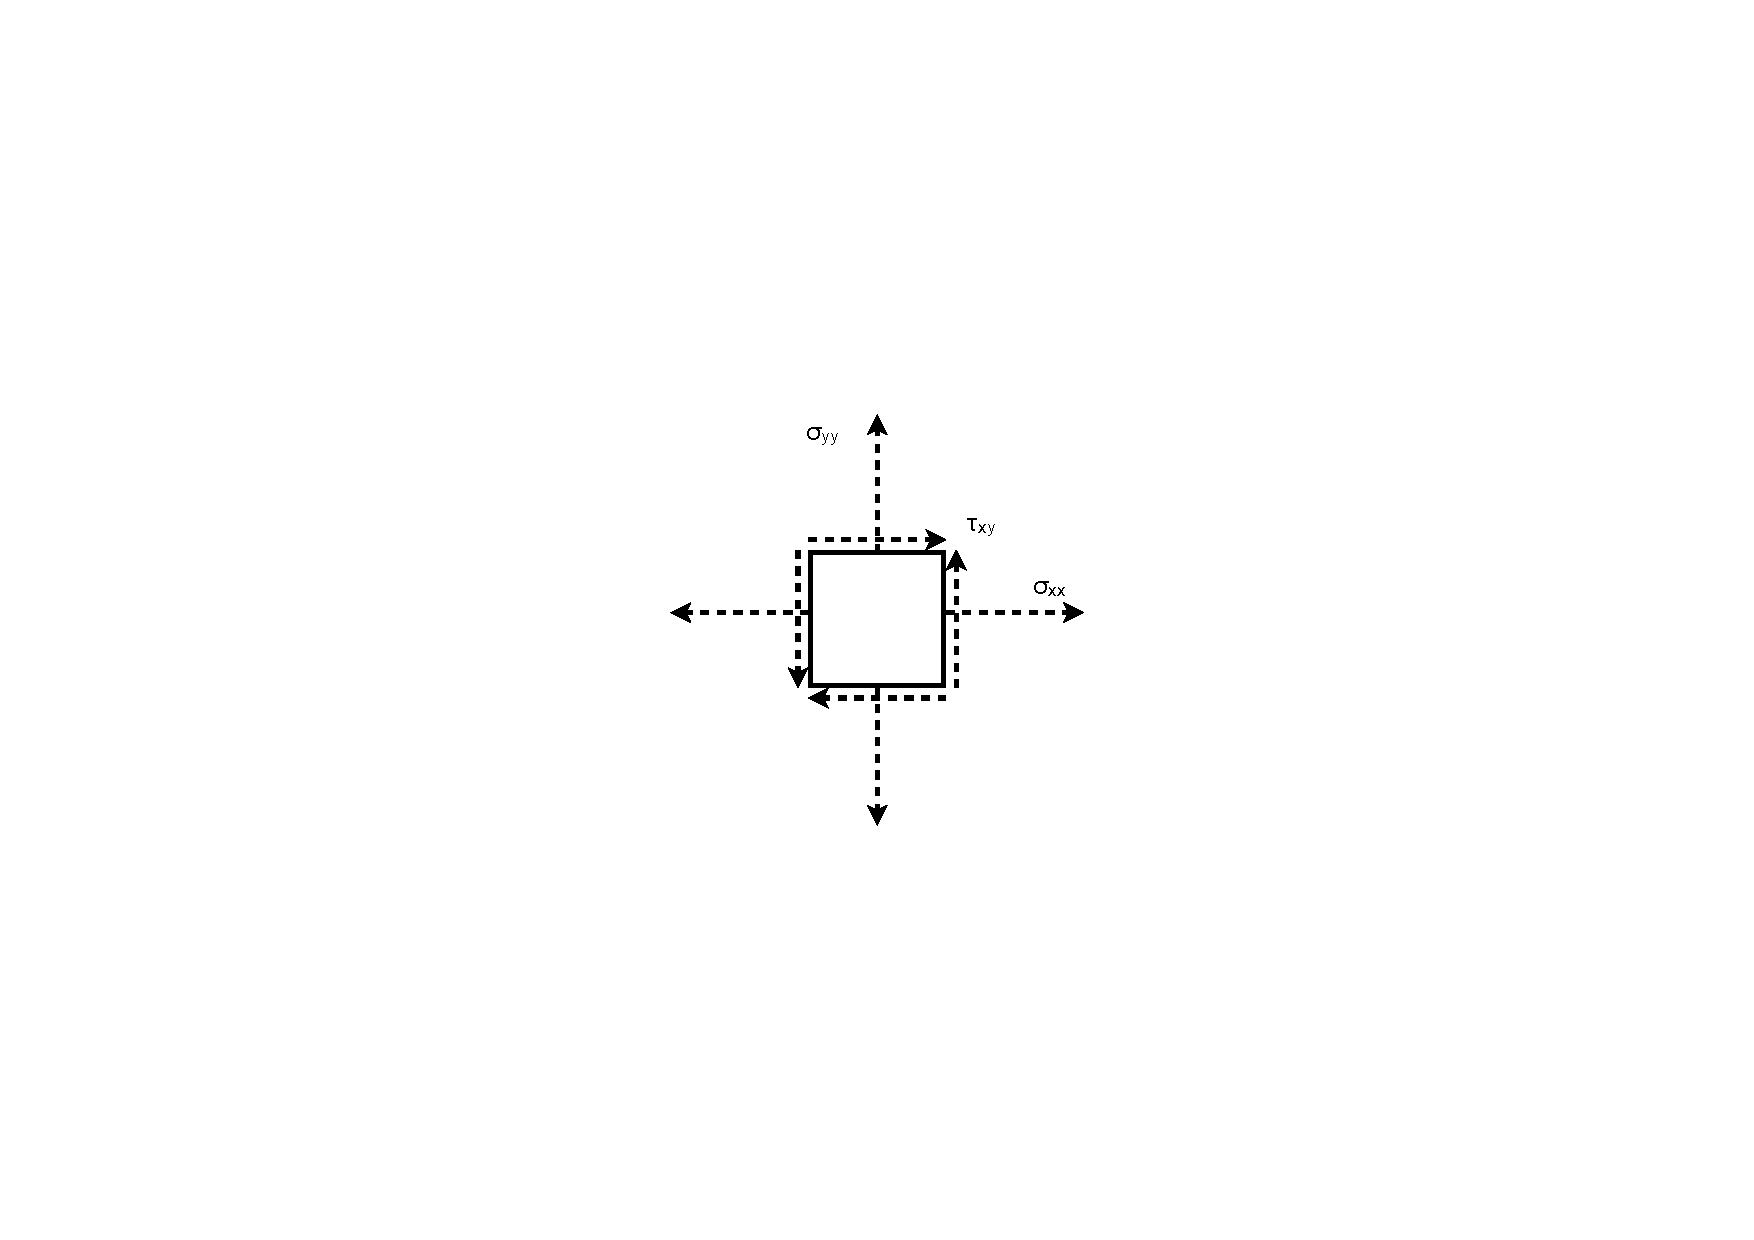
\includegraphics[width=0.45\linewidth]{Graphics/Additional-Ex/2D-stress}
	\caption{A \twod state of stress at a point in a loaded material}
	\label{fig:2D-stress}
\end{figure}
The maximum and minimum normal stresses (principal stresses) at the point, $\sigma_{\textrm{max}}$ and $\sigma_{\textrm{min}}$, are calculated from the stress components by:
\begin{equation*}
\sigma_{\textrm{max} \atop \textrm{min}} = \frac{\sigma_{xx}+\sigma_{yy}}{2} \pm \sqrt{{\left( \frac{\sigma_{xx}-\sigma_{yy}}{2} \right)}^2 + \tau_{xy}^2}
\end{equation*}
Write a user-defined function that determines the principal stresses from the stress components. For the function name and arguments use \mcode{[Smax,Smin] = princstress(Sxx,Syy,Sxy)}. Use the function to determine the principal stresses for the following states of stress: $\sigma_{xx} = -190~MPa$, $\sigma_{yy} = 145~MPa$, $\tau_{xy} = 110~MPa$.

\newpage
\item \textit{Functions}\\
In a low-pass RC filter (a filter that passes signals with low frequencies), the ratio of the magnitude of the voltages is given by:
\begin{equation*}
RV = \left| \frac{V_o}{V_i} \right| = \frac{1}{\sqrt{1+(\omega RC)^2}},
\end{equation*}
where $\omega$ is the frequency of the input signal. 
\begin{figure}[h]
	\myfloatalign
	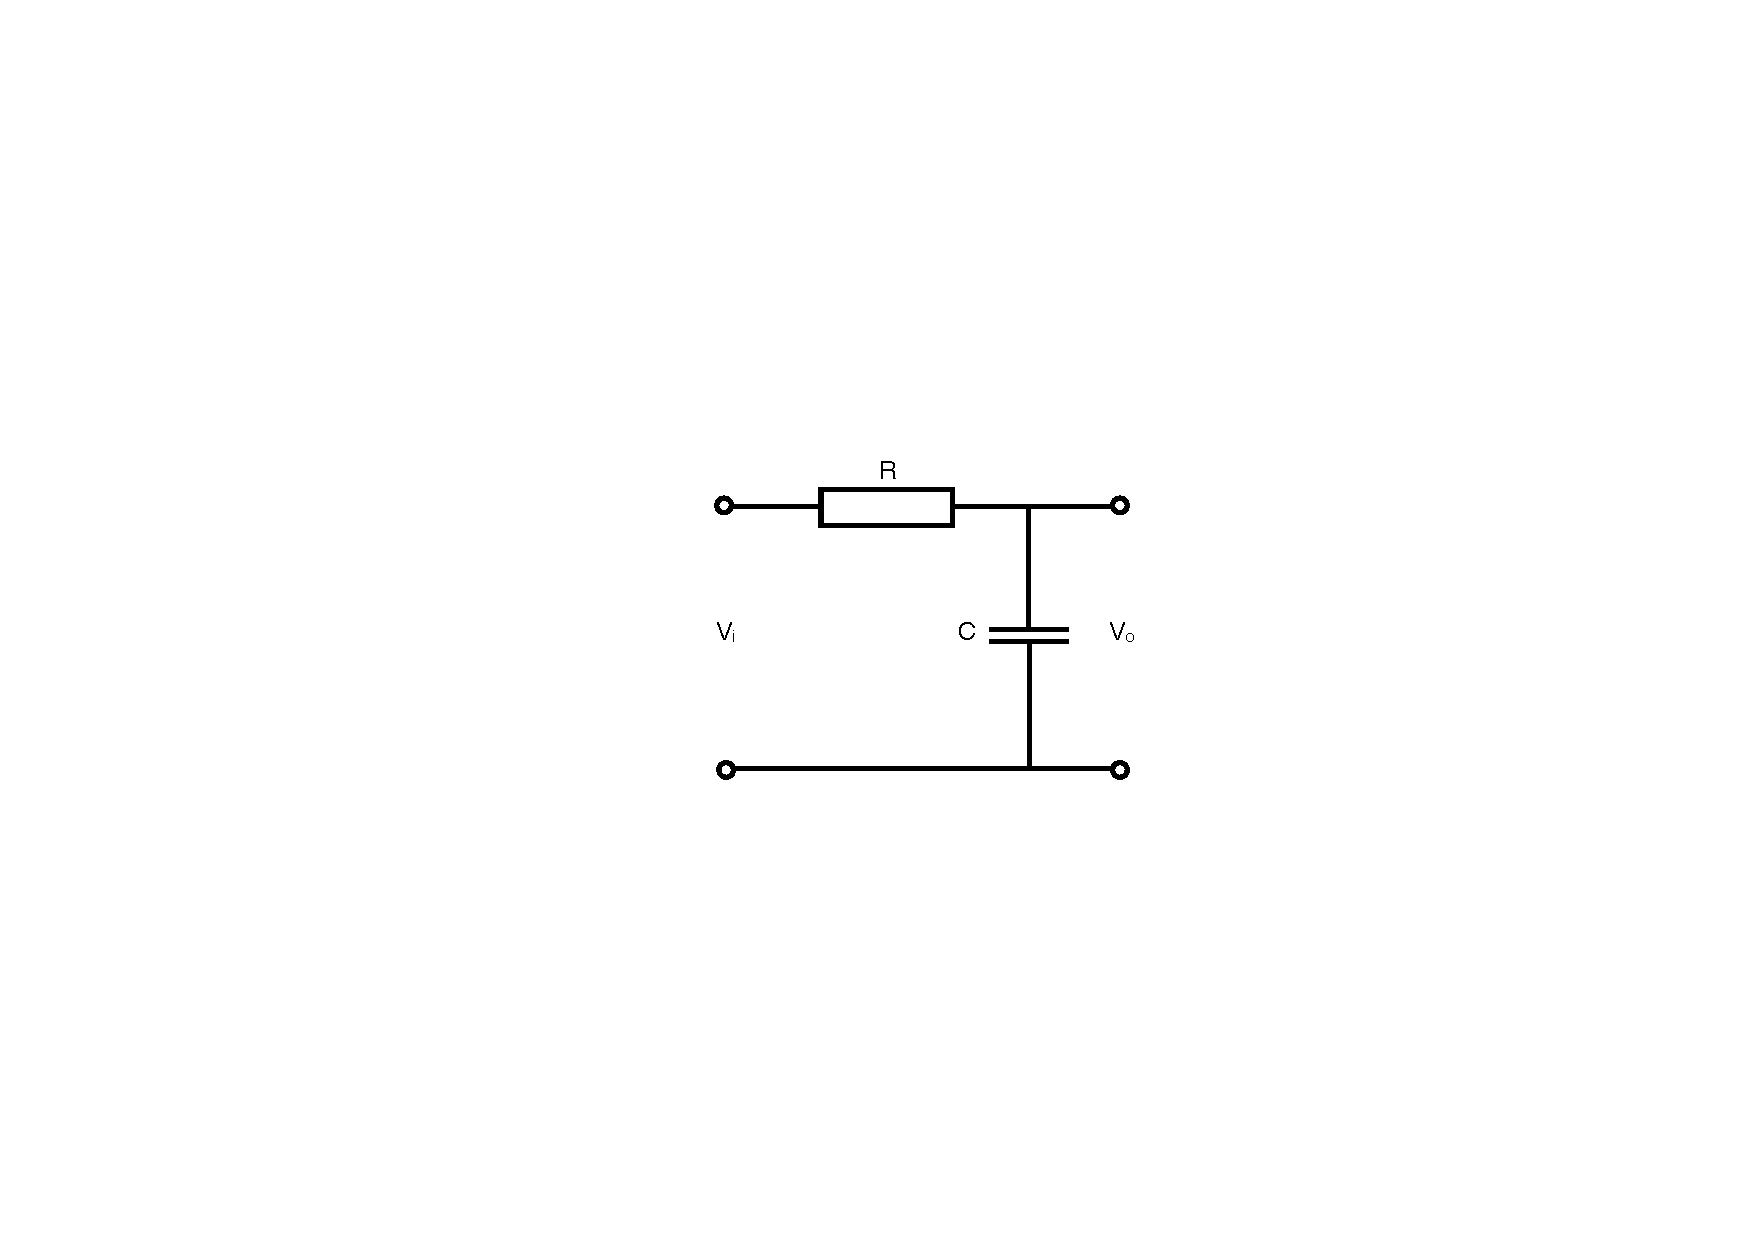
\includegraphics[width=0.55\linewidth]{Graphics/Additional-Ex/lowpass}
	\caption{A low-pass filter}
	\label{fig:lowpass}
\end{figure}
Write a user-defined function that calculates the magnitude ratio. For the function name and arguments use \mcode{RV = lowpass(R,C,w)}. The input arguments are: \mcode{R} the size of the resistor in $\Omega$ (ohms), \mcode{C} the size of the capacitor in $F$ (Farads), and \mcode{w} the frequency of the input signal in $rad/s$. Write the function such that \mcode{w} can be a vector.

Write a script file that uses your \mcode{lowpass} function to generate a plot of $RV$ as a function of $\omega$ for $10^{-2}\leq \omega \leq 10^6~rad/s$. The plot should have a logarithmic scale on the x-axis ($\omega$). When the script file is executed it should prompt the user to enter values of $R$ and $C$. Run the script file with $R=1200~\Omega$ and $C=8~\mu F$.

\newpage
\section{Decision Making} \label{sect:decisions}
\item \textit{Relational \& Logical operators}\\
The following were the daily maximum temperatures ($^\circ C$) in Washington DC during the month of April 2002: 14, 23, 23, 12, 10, 9, 13, 23, 23, 19, 21, 17, 23, 28, 29, 33, 34, 32, 33, 27, 15, 21, 13, 18, 17, 19, 18, 23, 17, 21. Write a script, and use relational and logical operators to determine the following:
\begin{enumerate}
\item The number of days the temperature was above $24~^\circ C$.
\item The number of days the temperature was between $18~^\circ C$ and $27~^\circ C$.
\end{enumerate}

%\item \textit{Relational \& Logical operators}\\
%The concentration of a drug in the body $C_p$ can be modelled by the equation:
%\begin{equation*}
%C_p = \frac{D_G}{V_d}\frac{k_a}{(k_a - k_e)}\left( e^{-k_e t} - e^{-k_a t} \right),
%\end{equation*}
%where $D_G$ is the dosage administered ($mg$), $V_d$ is the volume of distribution ($L$), $k_a$ is the absorption rate constant ($h^{-1}$), $k_e$ is the elimination rate constant ($h^{-1}$), and $t$ is the time ($h$) since the drug was administered. For a certain drug, the following quantities are given: $D_G=150~mg$, $V_d=50~L$, $k_a=1.6~h^{-1}$, and $k_e=0.4~h^{-1}$. A single dose is administered at $t=0$. Write a script to calculate and plot $C_p$ versus $t$ for 10~hours.

%\newpage
%\section{Loops} \label{sect:loops}
%\item \textit{\mcode{for} loops and \mcode{if} statements}\\
%The concentration of a drug in the body $C_p$ can be modelled by the equation:
%\begin{equation*}
%C_p = \frac{D_G}{V_d}\frac{k_a}{(k_a - k_e)}\left( e^{-k_e t} - e^{-k_a t} \right),
%\end{equation*}
%where $D_G$ is the dosage administered ($mg$), $V_d$ is the volume of distribution ($L$), $k_a$ is the absorption rate constant ($h^{-1}$), $k_e$ is the elimination rate constant  ($h^{-1}$), and $t$ is the time ($h$) since the drug was administered. For a certain drug, the following quantities are given: $D_G=150~mg$, $V_d=50~L$, $k_a=1.6~h^{-1}$, and $k_e=0.4~h^{-1}$. A first dose is administered at $t=0$, and subsequently four more doses are administered at intervals of four hours (\ie\ at $t=4,8,12,16$). Write a script to calculate and plot $C_p$ versus $t$ for 24~hours.

\item \textit{\mcode{while} loops}\\
The flight of a model rocket of mass 0.05~kg can be modelled as follows. During the first 0.15~s the rocket is propelled up by the rocket engine with a force of 16~N. The rocket then flies up slowing down under the force of gravity. After it reaches the apex, the rocket starts to fall back down. When its down velocity reaches 20~m/s a parachute opens (assumed to open instantly) and the rocket continues to move down at a constant speed of 20~m/s until it hits the ground. Write a script that calculates and plots the speed and altitude of the rocket as a function of time during the flight.
\begin{figure}[h]
	\myfloatalign
	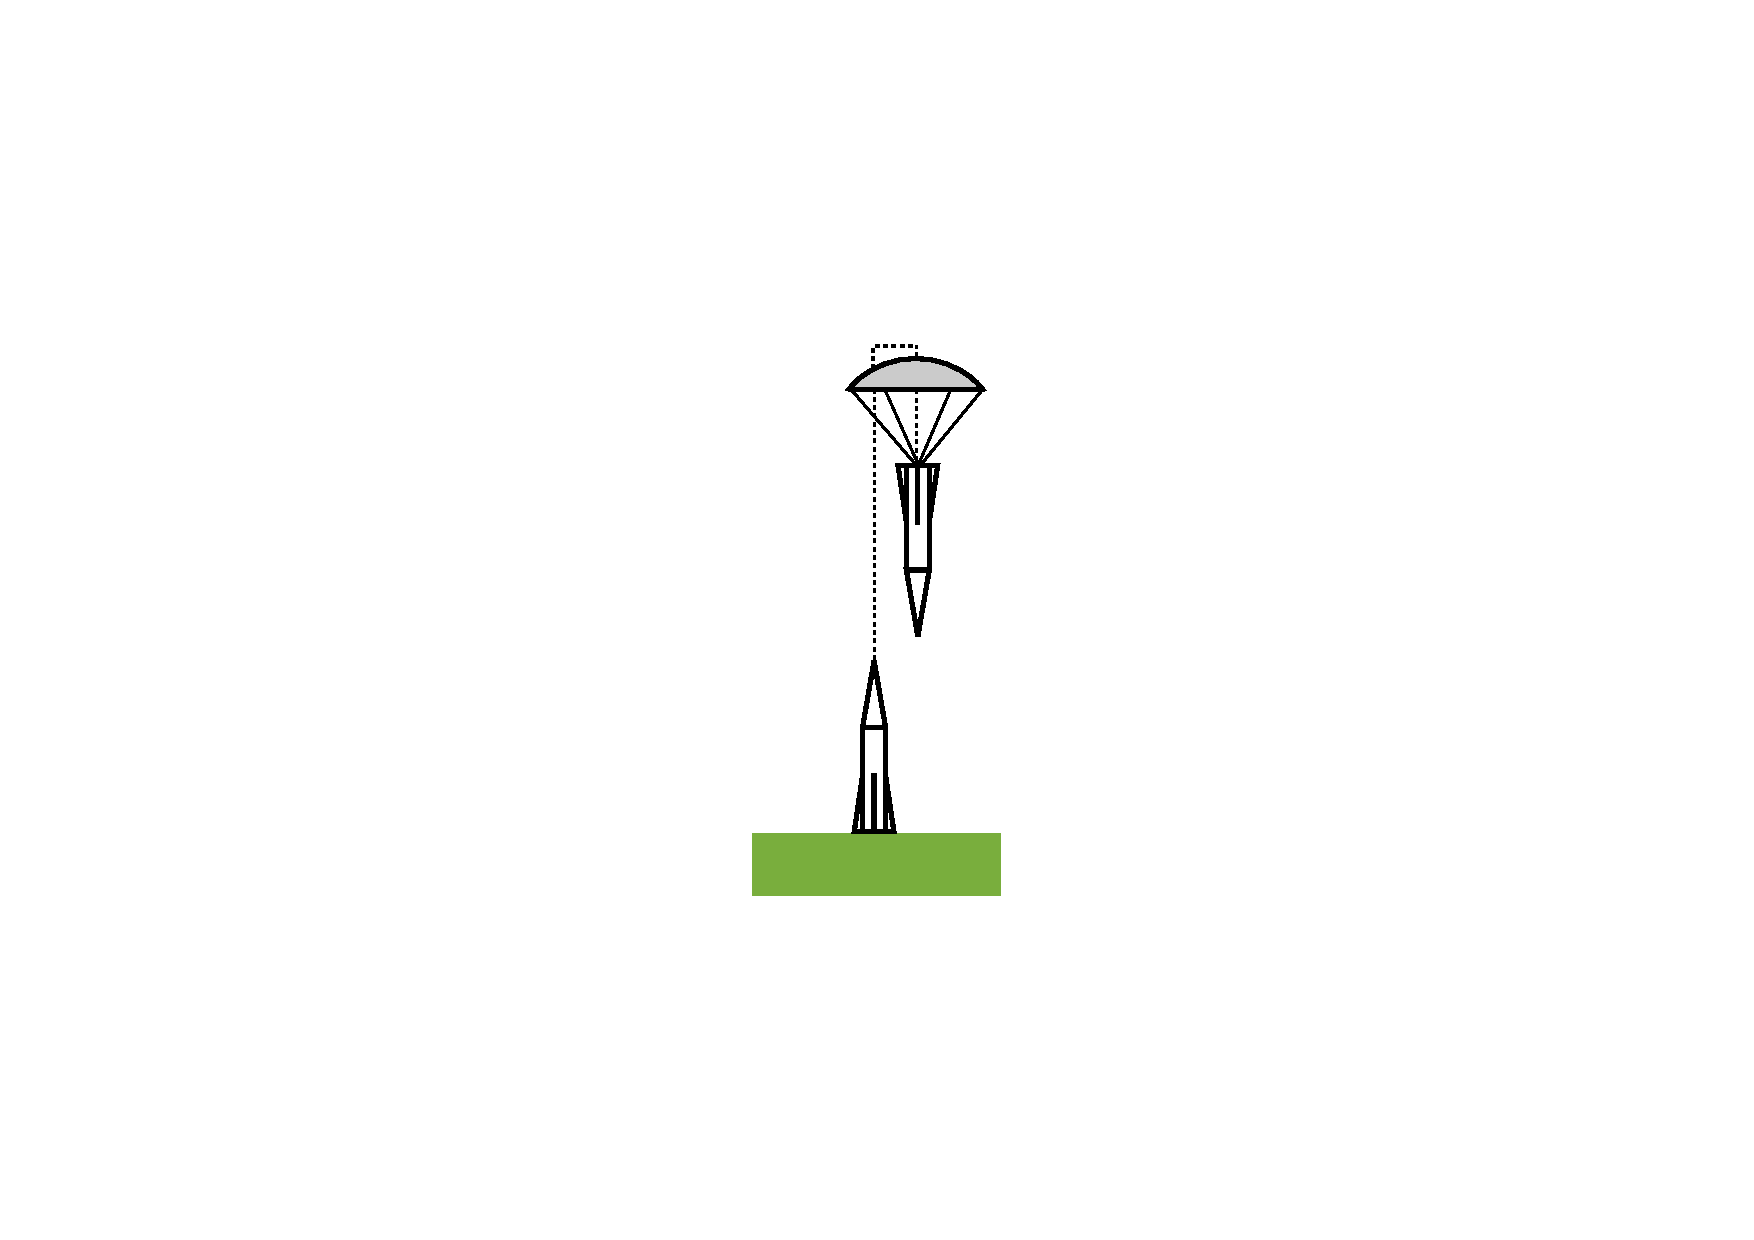
\includegraphics[width=0.15\linewidth]{Graphics/Additional-Ex/rocket}
	\caption{Flight of a model rocket}
	\label{fig:rocket}
\end{figure}

\addtolength{\parindent}{-4mm}
\fcolorbox{myborderblue}{myblue}{%
\begin{minipage}{\linewidth}
\begin{minipage}{6mm}

\includegraphics[scale=0.03]{Graphics/General/help_icon}
\end{minipage}
\textit{Flight of a model rocket}\\
The rocket is assumed to be a particle that moves along a straight line in the vertical plane. For motion with constant acceleration along a straight line, the velocity and position as a function of time are given by:
\begin{equation*}
v(t) = v_0 + at \quad \textrm{and} \quad s(t) = s_0 + v_0t + \frac{1}{2}at,
\end{equation*}
where $v_0$ and $s_0$ are the initial velocity and position, respectively.
The flight of the rocket can be divided into three segments and you should calculate each segment using a separate \mcode{while} loop in your script.\\

\textit{Segment 1 - The first 0.15~s when the rocket engine is on}\\
During this period, the rocket moves up with a constant acceleration. The acceleration is determined by drawing a free body and a mass acceleration diagram. From Newton's second law, summing the forces in the vertical direction gives an equation for the acceleration:
\begin{equation*}
a = \frac{F_E - mg}{m}
\end{equation*}
The velocity and height as a function of time are:
\begin{equation*}
v(t) = 0 + at \quad \textrm{and} \quad h(t) = 0 + 0 + \frac{1}{2}at^2,
\end{equation*}
where the initial velocity and initial position are both zero. In your script this \mcode{while} loop starts at $t=0$ and continues looping as long as $t\leq 0.15~s$. The time, velocity and height at the end of this segment are $t_1$, $v_1$, and $h_1$.\\

\textit{Segment 2 - The motion from when the engines stops until the parachute opens}\\
In this segment the rocket moves with a constant deceleration $g$. The speed and height of the rocket as a function of time are given by:
\begin{equation*}
v(t) = v_1 - g(t-t_1) \quad \textrm{and} \quad h(t) = h_1 + v_1(t-t_1) - \frac{1}{2}g(t-t_1)^2
\end{equation*}
In your script this \mcode{while} loop should continue looping until the velocity of the rocket is $-20~m/s$ (negative since the rocket is falling). The time and height at the end of this segment are $t_2$ and $h_2$.
\end{minipage}%
}\\

\addtolength{\parindent}{4mm}
\addtolength{\parindent}{-4mm}
\fcolorbox{myborderblue}{myblue}{%
\begin{minipage}{\linewidth}
\begin{minipage}{6mm}

\includegraphics[scale=0.03]{Graphics/General/help_icon}
\end{minipage}
\textit{Flight of a model rocket \textit{(continued)}}\\
\textit{Segment 3 - The motion from when the parachute opens until the rocket hits the ground}\\
In this segment the rocket moves with constant velocity (zero acceleration). The height as a function of time is given by:
\begin{equation*}
h(t) = h_2 + v_{\textrm{chute}}(t-t_2),
\end{equation*}
where $v_{\textrm{chute}}$ is the constant velocity after the parachute opens. In your script this \mcode{while} loop should continue looping as long as the height is greater than zero.
\end{minipage}%
}\\
\addtolength{\parindent}{4mm}

\end{enumerate}
